
\documentclass[12pt]{article}

% ----------- Packages -----------
\usepackage[a4paper, margin=2.5cm]{geometry}
\usepackage{graphicx} % for images
\usepackage{amsmath, amssymb} % for math
\usepackage{physics} % for physics
\usepackage{siunitx} % for units
\usepackage{caption}
\usepackage{tikz} %diagrams
\usetikzlibrary{arrows.meta, decorations.pathmorphing, patterns, bending, calc, positioning}
\usepackage{fancyhdr} % for header/footer
\usepackage{setspace} % for spacing
\usepackage{titlesec} % custom section titles
\usepackage{hyperref} % for hyperlinks
\usepackage{float} % for figure positioning
\usepackage{tocloft} % formatting ToC
\usepackage[backend=biber, style=apa]{biblatex} % references
\usepackage{hyperref} % href
\usepackage[capitalise, nameinlink]{cleveref} % links to sections
\usepackage{forest} % file directory trees
\usepackage{tabularx} % tables
\usepackage{fontspec} % font
\usepackage{float} % positioning
\usepackage{enumitem} % lists
\usepackage{xcolor} % color
\usepackage{wasysym} % diameter
\usepackage{pgfplotstable} % imported tables
\usepackage{booktabs} % better tables
\usepackage{siunitx} % math formatting in tables
\usepackage{tcolorbox} % terminal like appearance
\usepackage{pgffor} % loops
\usepackage{subcaption} % images with loop
\usepackage{listings} % code

\addbibresource{references.bib}  
% ----------- Settings -----------
\setmainfont{Times New Roman}
\setmonofont{Lucida Console}[Scale=MatchLowercase]

\tcbuselibrary{listings}

\lstset{
	language=Python,
	basicstyle=\ttfamily\small,
	keywordstyle=\color{blue},
	commentstyle=\color{gray},
	stringstyle=\color{orange},
	numbers=left,
	numberstyle=\tiny,
	stepnumber=1,
	numbersep=5pt,
	showstringspaces=false,
	breaklines=true,
	breakatwhitespace=false,
	frame=single,
	captionpos=b
}

% ----------- Title Page -----------


% ----------------------------------
\begin{document}

\begin{titlepage}
	\begin{center}
		\textbf{Extended Essay: Physics}
		
		\vspace*{4cm}
		
		\textbf{Title:}\
		The Relationship Between Polygon Geometry and Vortex Shedding Frequency in a Two-Dimensional Laminar Flow
		\vspace{1cm}
		
		\textbf{RQ:}\
		How does increasing the number of faces of a bluff body (ranging from 2 to 12) affect the vortex shedding frequency in laminar flow, measured in Hz, in a two-dimensional plane?
		\vspace{4cm}
		
		Word count:
		
		\ldots
		\vfill
		
		\vspace{0.1cm}
	\end{center}
\end{titlepage}
	
	
\tableofcontents
\newpage
	
\section{Introduction}

Despite its widespread significance, the study of fluid dynamics is largely overlooked by the IB Physics syllabus. Defined as a field of applied science dedicated to studying the motion and interaction of fluid substances, fluid dynamics is one of the two sub-fields of fluid mechanics, the field concerned with understanding the dynamics of fluids subject to external forces \parencite{livescience_fluid_dynamics}. 

From the air we breathe to the water we consume; fluids are present in almost every aspect of our lives. Although observing fluids in action is a daily occurrence for all, countless remain unaware of the highly complex and intricate theories governing these seemingly simple and elementary phenomena. Ultimately, a profound youthful interest in cars and planes \textemdash\ everything with an engine really \textemdash\ coupled with a fascination for the motion of fluids led to the topic of this essay: vortex shedding. Specifically, this essay will concern itself with the question: \textit{How does increasing the number of streamwise faces of a bluff body (ranging from 2 to 12) affect the vortex shedding frequency in laminar flow, measured in Hz, in a 2D plane?}

Over the past century, vortex shedding has garnered a multifold of attention, with hundreds of papers published \parencite[61]{buresti1998}. This partially elucidated phenomenon is quintessential in a broad range of scientific and engineering contexts, from maintaining ubiquitous infrastructure to developing cutting-edge aerospace technologies. Bridges may suffer from vortex shedding excitation, a severe challenge which undermines their structural integrity \parencite[1040]{jurado2012}. This was exemplified by the collapse of the Tacoma Narrows Bridge on the 7th of November 1940, where vortex shedding acted as the instigating mechanism -- triggering vertical vibration that eventually transitioned into the torsional oscillations, ultimately causing its collapse \parencite{tacoma_bridge_vibrations}.

As previously mentioned, the IB Physics Guide \parencite{ib_physics_2025} does not directly concern itself with vortex shedding or, in general, the majority of fluid dynamics. Nevertheless, links can be made to section C: "Wave Behavior". Section C.1, "Simple Harmonic Motion", concerns itself with, as the name suggests, simple harmonic motion, an idealized theoretical representation of the behavior of oscillatory systems \parencite[313]{allum2023}. Fundamental concepts such as frequency and time period are discussed, ideas required in order to analyze the frequency of the vortex shedding caused by a bluff body. Furthermore, the topic of this essay also links to section C.4, "Standing Waves and Resonance". Concepts of natural frequency, vibrations and resonance are key when discussing the problems caused by vortex shedding, like the one detailed above, and the significance of the frequency of vortex shedding. 






\section{Background}

\subsection{Fundamentals of Fluid Dynamics}
Firstly, the definition of vorticity, a vortex and a bluff body must be understood. \textbf{Vorticity} is the vector quantity representing the rotational motion in a velocity field \parencite[p.~2500]{holton2003_vorticity}. A \textbf{vortex} is the circular flow of a fluid around a central axis, characterized by the vorticity in the fluid \parencite[p.~390]{nitsche2006_vortex}. A \textbf{bluff body} is defined as an object that, due to its geometry, induces significant regions of separated flow \parencite[p.~561]{navalhydro1997}. 

Next, one must distinguish between a Newtonian and a non-Newtonian fluid. A \textbf{Newtonian fluid} is a fluid in which the viscosity -- a measure of internal friction -- remains constant despite applied shear rate, whereas a \textbf{non-Newtonian} fluid exhibits a viscosity which varies with the applied force \parencite{mohn2024}. 

Moreover, one must also consider the type of flow. There are two key factors of flow when investigating vortex shedding: laminar and turbulent flow, and compressible and incompressible flow. \textbf{Laminar flow} is characterized by the layered motion of fluid particles, with no significant disturbance between the parallel layers \parencite[pp.~40--41]{versteeg2007}. On the other hand, \textbf{turbulent flow} is known to have continuous, irregular fluctuations in velocity and pressure throughout the fluid \parencite[p.~40]{versteeg2007}. A \textbf{compressible flow} is a flow in which the fluid does not have a uniform density \parencite[p.~31]{oran2002}, conversely, an \textbf{incompressible flow} is a flow in which the fluid has a constant density \parencite[p.~12]{versteeg2007}. 

This essay will analyze vortex shedding in a Newtonian fluid – water – which exhibits laminar and incompressible flow.

Lastly, two dimensionless numbers must be considered: the Reynolds and Strouhal number. The \textbf{Reynolds number} expresses the “ratio between inertial and viscous forces” \parencite{nasa_reynolds}. Given by the equation 
\[
\mathrm{Re} = \frac{\rho U L}{\mu}
\]
where $\rho$ is the density of the fluid ($kg\,m^{-3}$), $U$ is the free-stream velocity ($m\,s^{-1}$), $L$ is the characteristic length ($m$) and $\mu$ is the dynamic viscosity ($kg\,m^{-1}\,s^{-1}$). This number allows one to classify if a flow is laminar or turbulent, with low Reynolds’ numbers signifying laminar flow and high Reynolds’ numbers indicating turbulent flow \parencite{saldana2024_reynolds}. The \textbf{Strouhal number} is a dimensionless parameter used to describe the periodicity of vortex shedding \parencite[p.~211]{choi2000strouhal}. It is given by the equation 
\[
\mathrm{St} = \frac{f L}{U}
\]
where $f$ is the frequency of vortex shedding ($Hz$), $L$ is the characteristic length ($m$) and $U$ is the free-stream velocity  ($m\,s^{-1}$). A high Strouhal number -- assuming both $L$ and $U$ remain constant -- indicates an increased vortex shedding frequency $f$, conversely a low Strouhal number indicates a lower $f$.


\subsection{Vortex Shedding and the Kármán Vortex Street}
Vortex shedding in a two-dimensional plane can be defined as the phenomenon in which localized regions of high vorticity are periodically released into the wake from alternating sides of a bluff body, each exhibiting an opposite rotational direction \parencite[156]{green1995fluid}. Whereas vortex shedding is the process by which vortices are formed, Kármán Vortex Street refers to the flow pattern created, a repeated structure of counter-rotating vortices \parencite[26]{govardhan2005karman}.

\begin{figure}[htbp]
	\centering
	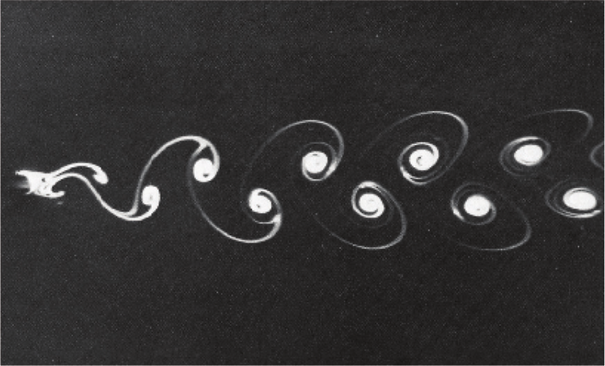
\includegraphics[width=0.7\textwidth]{images/vonKarmanStreet.png}
	\caption{Von Kármán Street behind a cylinder in a non-rotating 2D flow for Re = 140, fluorescein visualization \parencite[144]{ilieva2017turbulence}}
	\label{fig:vonKarmanStreet}
\end{figure}
\subsection{The Mechanism of Vortex Shedding}
Due to the fiction between a given fluid and a bluff body, there is no relative motion between them \parencite{boundaryLayerTheory_2018, jeff_defoe_bluff_2020}. Consequently, if the velocity of the bluff body is zero, the velocity of the fluid at the wall of the bluff body, with respect to the reference frame of the bluff body, is also zero: a no-slip condition. This causes a variation in velocities with distance, from zero at the bluff body surface to the free stream velocity U at a certain distance from the bluff body. The region in which this velocity gradient occurs is referred to as the boundary layer.

\pgfdeclarelayer{background}
\pgfdeclarelayer{foreground}
\pgfsetlayers{background,main,foreground}

\begin{figure}[H]
	\begin{center}
		\begin{tikzpicture}[scale=1.2]
			
			% Axes
			\draw[->, ultra thick] (0,0) -- (0,6) node[above] {Distance from wall, $y$};
			\begin{pgfonlayer}{foreground}
				\draw[->, ultra thick] (0,0) -- (5.5,0) node[right] {$u$};
			\end{pgfonlayer}
			
			% Wall
			\filldraw[lightgray] (-2,-0.2) rectangle (4.8, 0);
			\node[anchor=east] at (-2, -0.1) {Face of bluff body};
			\node[anchor=north] at (2, -0.7) {No-slip condition};
			\draw[->, anchor=north] (0.7, -0.7) -- (0.05, -0.05);
			
			% Boundary layer thickness
			\draw[dashed] (-1,5) -- (2.5,5);
			\draw[<->, thick] (-0.4,0) -- (-0.4,5);
			\node[anchor=east] at (-0.5,2.5) {Boundary layer thickness, $\delta$};
			
			% External flow
			\draw[->, thick, blue] (0,5) -- (2.5,5);
			\node[blue] at (2.8,5) {$U$};
			\node[blue, anchor=south] at (1.3,5.05) {\footnotesize Free flow velocity};
			
			% Curve
			\draw[thick](0,0)
			.. controls (2, 0.6) and (2.5, 1.2) .. (2.5, 5); 
			
			% Arrows
			\draw[->] (0,0.5) -- (1.2, 0.5);
			\draw[->] (0,1) -- (1.8, 1);
			\draw[->] (0, 1.5) -- (2.1, 1.5);
			\draw[->] (0,2) -- (2.25, 2);
			\draw[->] (0, 2.5) -- (2.35, 2.5);
			\draw[->] (0,3) -- (2.41, 3);
			\draw[->] (0, 3.5) -- (2.46, 3.5);
			\draw[->] (0,4) -- (2.5, 4);
			\draw[->] (0, 4.5) -- (2.51, 4.5);
			
			% Velocity profile label
			\node[anchor=west] at (3.5,2.3) {Velocity profile,};
			\node[anchor=west] at (3.5,2) {$u = u(y)$};
			\draw[->, anchor=east] (3.5, 2.3) -- (2.5, 2.8);
			
		\end{tikzpicture}
	\end{center}
	\caption{Depiction of boundary layer and the velocity gradient formed. Inspired by \textcite{erau_boundarylayer}}
	\label{fig:boundaryLayer}
\end{figure}

When a flow moves past a bluff body in a two-dimensional plane, a boundary layer develops, with increasing thickness from the stagnation point \parencite{fitzpatrick2016_reynolds}, the point on the leading edge of the bluff body at which the local fluid velocity is zero (with respect to the bluff body), to the back of the bluff body \parencite{learneng2022_boundarylayer}. At a certain point, the boundary layer separates from the bluff body, forming a shear layer. Under steady flow conditions, this separation occurs in a periodic and alternating manner, creating two separate, out-of-phase shear layers on either side of the bluff body. 

\begin{figure}[H]
	\begin{center}
		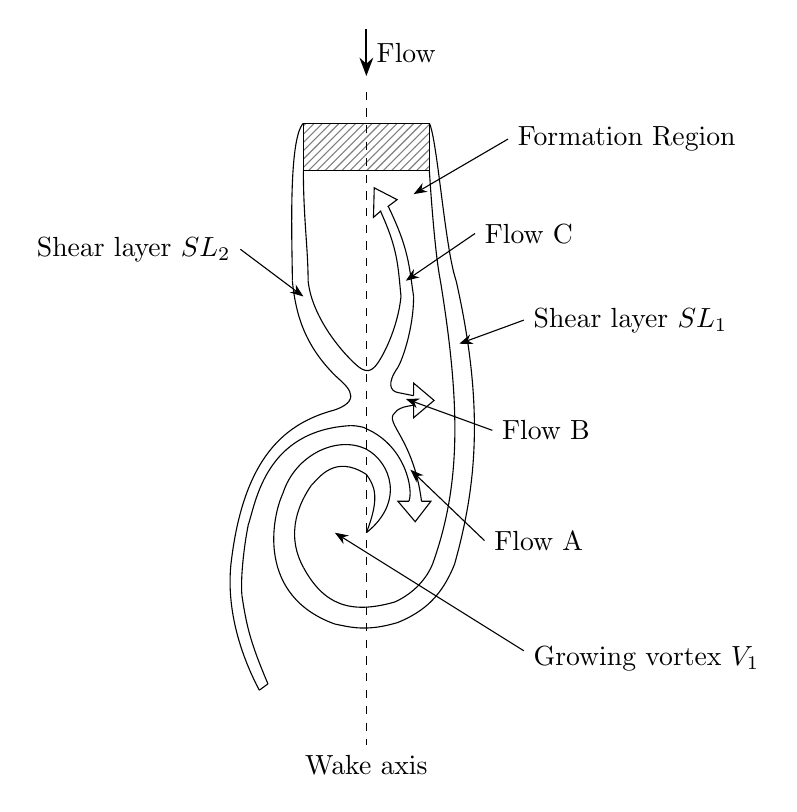
\begin{tikzpicture}[scale=0.2, >=Stealth]
			
			% Main vertical flow arrow
			\draw[->, thick] (0,39) -- (0,36) node[midway, right] {Flow};
			
			% Obstacle rectangle
			\draw[pattern=north east lines, pattern color=black!50] (-4,33) rectangle (4,30);
			
			% Shear layers 
			\draw (-4, 33)
			.. controls (-5, 32) and (-4.7, 25) .. (-4.7, 23);
			\draw (-4.7, 23)
			.. controls (-4.5, 21) and (-4, 19) .. (-2, 17);
			\draw (-2,17)
			.. controls (-1.5, 16.5) and (0, 15.5) .. (-2, 14.8);
			\draw (-2, 14.8)
			.. controls (-5, 14) and (-7.8, 12) .. (-8.6, 5);
			\draw (-8.6, 5)
			.. controls (-8.7, 4) and (-8.9, 1) .. (-6.8, -3);
			
			
			\draw (-4, 30)
			.. controls (-4, 27) and (-3.7, 25) .. (-3.7, 23);
			\draw (-3.7, 23)
			.. controls (-3.5, 21) and (-2, 19) .. (-1, 18);
			\draw (-1,18)
			.. controls (-0.5, 17.5) and (0, 17) .. (0.5, 17.5);
			\draw (0.5, 17.5)
			.. controls (1, 18) and (2, 20) .. (2.2, 22);
			\draw (2.2, 22)
			.. controls (2, 24) and (2, 25) .. (0.9, 27.41);
			
			
			\begin{scope}[shift={(-0.3,7.9)}]
				\draw (1.24,19.55) -- (0.75 ,19.125) -- (0.8,21) -- (2.25,20.25) -- (1.65,19.8);
			\end{scope}
			
			
			\draw (2, 17.5)
			.. controls (2.3, 18) and (3, 20) .. (3, 22);
			\draw (3, 22)
			.. controls (2.7, 24) and (2.7, 25) .. (1.4, 27.7);
			
			
			\draw (2, 17.5)
			.. controls (1.3, 16.5) and (1.5, 16) .. (2, 15.9);
			
			
			\draw (2, 15.9) -- (3, 15.7);
			
			
			\draw (3, 15.7) -- (3, 16.5) -- (4.3, 15.4) -- (3, 14.3) -- (3, 15.1);
			
			
			\draw (3, 15.1)
			.. controls (2.5, 15) and (2.1, 15) .. (1.8, 14.6);
			
			
			\draw (1.8, 14.6)
			.. controls (1.1, 14) and (3, 13) .. (3.5, 9);
			
			
			\draw (3.5, 9) -- (4.1, 9) -- (3.1, 7.7) -- (2, 9) -- (2.7, 9);
			
			
			\draw (2.7, 9)
			.. controls (3, 9.7) and (2.5, 12.5) .. (0, 13.6);
			\draw (0, 13.6)
			.. controls (-0.3, 13.8) and (-1, 13.8) .. (-1, 13.8);
			
			
			\draw (-1, 13.8)
			.. controls (-6.4, 13.5) and (-7, 9) .. (-7.5, 7.5);
			\draw (-7.5, 7.5)
			.. controls (-7.8, 6) and (-8, 4) .. (-7.9, 3);
			\draw (-7.9, 3)
			.. controls (-7.6, 1) and (-7.35, 0) .. (-6.25, -2.6);
			\draw (-6.8, -3) -- (-6.25, -2.6);
			
			
			
			\draw (4, 33)
			.. controls (4.5, 32) and (5, 25) .. (5.7, 23);
			\draw (5.7, 23)
			.. controls (7.5, 15) and (7, 10) .. (5.6, 5);
			\draw (5.6, 5)
			.. controls (4.8, 3) and (3.7, 2) .. (2, 1.3);
			\draw (2, 1.3)
			.. controls (0, 0.7) and (-1, 1) .. (-2, 1.2);
			\draw (-2, 1.2)
			.. controls (-7, 3) and (-6, 8) .. (-5.3, 9.5);
			\draw (-5.3, 9.5)
			.. controls (-4.5, 12) and (-1.8, 13.2) .. (0, 12.3);
			\draw(0, 12.3)
			.. controls (1.5, 11.5) and (2.5, 9) .. (0, 7);
			
			\draw (4, 30)
			.. controls (4, 30) and (4.3, 25) .. (4.7, 23);
			\draw (4.7, 23)
			.. controls (6, 15) and (6, 10) .. (4.2, 5);
			\draw (4.2, 5)
			.. controls (3.7, 3.8) and (2.7, 3) .. (1.8, 2.6);
			\draw (1.8, 2.6)
			.. controls (-1, 1.8) and (-2.7, 2.4) .. (-4, 4.8);
			\draw (-4, 4.8)
			.. controls (-5.2, 7) and (-4.2, 9) .. (-3.5, 10);
			\draw (-3.5, 10)
			.. controls (-3, 10.5) and (-2, 12) .. (0, 10.7);
			\draw(0, 10.7)
			.. controls (0.5, 10) and (0.9, 9.3) .. (0, 7);
			
			\node[anchor=west] at (6.9,26) {Flow C};
			\draw[->] (6.9, 26) -- (2.5, 23);
			
			\node[anchor=west] at (9,32) {Formation Region};
			\draw[->] (9, 32) -- (3, 28.5);
			
			\node[anchor=west] at (8,13.5) {Flow B};
			\draw[->] (8, 13.5) -- (2.5, 15.5);
			
			\node[anchor=west] at (7.5,6.5) {Flow A};
			\draw[->] (7.5, 6.5) -- (2.8, 11);
			
			\node[anchor=east] at (-8,25) {Shear layer $SL_2$};
			\draw[->] (-8, 25) -- (-4, 22);
			
			\node[anchor=west] at (10,20.5) {Shear layer $SL_1$};
			\draw[->] (10, 20.5) -- (5.9, 19);
			
			\node[anchor=north] at (0,-6.5) {Wake axis};
			
			\node[anchor=west] at (10,-1) {Growing vortex $V_1$};
			\draw[->] (10, -0.5) -- (-2, 7);
			
			% Wake axis dashed line
			\draw[dashed] (0,35) -- (0,-6.5);
			
		\end{tikzpicture}
	\end{center}
	\caption{The mechanism of vortex shedding. Inspired by \textcite[3]{shen2010_vortexmeter}}
	\label{fig:mechanismOfVortexShedding}
\end{figure}

For simplification, assume the first shear layer is generated at the right of the bluff body ($SL_{1}$). Due to its vorticity, the shear layer tends to curl up, forming a vortex. As the vortex forms, the pressure in the core of the vortex decreases, acting as a sink, inducing inflow towards its center. The fluid initially present at the bottom of the backside of the bluff body is drawn into the vortex, creating space, allowing for the formation of the left shear layer ($SL_{2}$) in the \textit{formation region}. This newly created shear layer splits into three distinct flows: a flow (\textit{Flow C}) which recirculates behind the bluff body, a flow (\textit{Flow B}) which mixes with the top shear layer and a flow (\textit{Flow A}) which is drawn into the vortex ($V_{1}$).

There is a decrease in strength of the vortex being created due to \textit{Flow A} having an opposite vorticity to the vorticity of the vortex. Moreover, the opposite vorticity of \textit{Flow B} and the right shear layer effectively nullifies each other, leading to the right shear layer being interrupted and the vortex becoming detached, causing it to travel with the main flow. The vortex has been “shed”. Since the vortex moves away from the bluff body, its low-pressure influence on the area near the bluff body decreases, allowing the left shear layer to more freely develop. Now, due to the periodic nature of vortex formation, the process recurs with the shear layers switching roles. 

When considering the vortex being created from the top shear layer, the fluid at the top of the vortex will have the same velocity as the free stream velocity U, whereas the velocity at the bottom of the vortex will be of a smaller magnitude and in the opposite direction of the main flow. According to Bernoulli’s equation, a region of higher velocity must have a lower pressure and vice versa. Therefore, the bottom region of the vortex will have a higher pressure than the top region, causing a lift force which acts on the bluff body normal to the flow. The oscillation of this lift force coincides with the vortex shedding frequency. 

\subsection{The Bluff Body}
\label{subsec:bluffBody}
In order to maintain a cylinder-like appearance, one of the most common bluff bodies investigated \parencite[475]{rocchi2002_vortex}, this investigation is conducted with bluff bodies which have a rectangular “tail”, in order to give each shape an equal overall length l\ in both streamwise and transverse directions.

\begin{figure}[H]
	\begin{center}
		\begin{tikzpicture}[line join=round, line cap=round, scale=0.7]
			
			% Base shape dimensions
			\def\W{4}   % width of the base
			\def\H{2}   % height of the base
			\def\R{2}   % roof "radius"
			
			% --- LEFT: 2-sided roof (n=2) ---
			\coordinate (A) at (0,0);
			\coordinate (B) at (\W,0);
			\draw (A) -- (B) -- (\W,\H)
			-- (\W/2,\H+\R) -- (0,\H) -- cycle;
			\node[below=8pt of $(A)!0.5!(B)$] {$n = 2$};
			
			% --- MIDDLE: 6-sided roof (n=6) ---
			\begin{scope}[xshift=7cm]
				\coordinate (A) at (0,0);
				\coordinate (B) at (\W,0);
				\draw (A) -- (B);
				\draw (A) -- (0,\H);
				\draw (B) -- (\W,\H);
				
				\foreach \k [evaluate=\k as \ang using {180 - 30*\k}] in {0,...,6}{
					\coordinate (m\k) at ({\W/2 + \R*cos(\ang)},
					{\H   + \R*sin(\ang)});
				}
				\draw (0,\H) -- (m0);
				\foreach \k in {0,...,5}{
					\pgfmathtruncatemacro\next{\k+1}
					\draw (m\k) -- (m\next);
				}
				\draw (m6) -- (\W,\H);
				\node[below=8pt of $(A)!0.5!(B)$] {$n = 6$};
			\end{scope}
			
			% --- RIGHT: 12-sided roof (n=12) ---
			\begin{scope}[xshift=14cm]
				\coordinate (A) at (0,0);
				\coordinate (B) at (\W,0);
				\draw (A) -- (B);
				\draw (A) -- (0,\H);
				\draw (B) -- (\W,\H);
				
				\foreach \k [evaluate=\k as \ang using {180 - 15*\k}] in {0,...,12}{
					\coordinate (r\k) at ({\W/2 + \R*cos(\ang)},
					{\H   + \R*sin(\ang)});
				}
				\draw (0,\H) -- (r0);
				\foreach \k in {0,...,11}{
					\pgfmathtruncatemacro\next{\k+1}
					\draw (r\k) -- (r\next);
				}
				\draw (r12) -- (\W,\H);
				\node[below=8pt of $(A)!0.5!(B)$] {$n = 12$};
			\end{scope}
			
		\end{tikzpicture}
	\end{center}
	\caption{Examples of bluff bodies}
	\label{fig:bluffBodies}
\end{figure}


\subsection{The Theoretical Investigation}
\subsubsection{Ansys Workbench}
The geometry and mesh preparation for the simulation was conducted using Ansys Workbench \parencite{noauthor_ansys_nodate}. The dimensions of the fluid domain are based on \ref{fig:fluidDomain} where l is the overall length of the bluff body.

\newlength\unitL
\setlength\unitL{0.2cm}

\begin{figure}[H]
	
	\begin{center}
		\begin{tikzpicture}[x=\unitL, y=\unitL, >=stealth, line width=1pt]
			
			% === Outer domain ===
			\draw (0,0) rectangle (63,50);
			
			% === Square obstacle ===
			\draw (22,24) rectangle (24,26);
			\draw[<->] (25, 24) -- (25, 26);
			\node at (27, 25) {$\ell$};  
			
			\draw[<->] (22, 23) -- (24, 23);
			\node at (23, 21) {$\ell$};  
			
			% === Velocity inlet arrows (spaced + farther from wall) ===
			\foreach \y in {12,20,28,36}
			\draw[->] (-5,\y) -- (-1,\y);  % stop at x=0.3 to add gap
			
			% === Velocity inlet label (more horizontal distance) ===
			\node[rotate=90] at (-7,25) {\large \textbf{Velocity Inlet}};
			
			% === Pressure outlet ===
			\draw[<->] (65.5,0) -- (65.5,50);
			\node[rotate=90] at (72,25) {\large \textbf{Pressure Outlet}};
			\node[rotate=90] at (68,25) {$50\,\ell$};
			
			% === Bottom dimensions (same horizontal alignment) ===
			\draw (23,0) -- (23,-0.8);  % tick at square center
			
			\draw[<->] (0,-3) -- (23,-3);  % from inlet to square center
			\node at (11.5,-5.1) {$23\,\ell$};
			
			\draw[<->] (23,-3) -- (63,-3); % from square center to outlet
			\node at (43,-5.1) {$40\,\ell$};
			
		\end{tikzpicture}
	\end{center}
	\caption{The fluid domain with dimensions. Inspired by \textcite{comflics_openfoam_2014}}
	\label{fig:fluidDomain}
\end{figure}

Given the computational limitations of the computer the simulation was conducted on, an overall length $\ell$ of $1\times{10}^{-3}$ meters was chosen, therefore giving each bluff body a characteristic length $L$ of $1\times{10}^{-3}$ meters. 

In order to create the mesh necessary for the simulation, the \textit{All Triangles Method} was utilized. A global unit size of $2.25\times{10}^{-3}$ meters was applied to the fluid domain to ensure a computationally inexpensive resolution in regions of negligible interest. Conversely, near the edge of the bluff body, a significantly smaller unit size of $2.0\times{10}^{-5}$ meters was used, constituting an accurate depiction of the interaction between the fluid flow and the bluff body \parencite{ansys_learning_best_2023}. Furthermore, eight inflation layers were employed in order to accurately capture the gradients associated with boundary layer formation at the edges of the bluff body \parencite{fluid_mechanics_101_cfd_2021}. Moreover, a body of influence (BOI) with a sizing of $2.0\times{10}^{-4}$ meters was used, positioned as shown in \ref{fig:fluidDomainWithBOI} below, in order to refine the mesh in the wake region, where the vortex shedding occurs, constituting for a more accurate simulation.  

\begin{figure}[H]

	\begin{center}
		\begin{tikzpicture}[x=\unitL, y=\unitL, >=stealth, line width=1pt]
			
			% === Outer domain ===
			\draw (0,0) rectangle (63,50);
			
			% === BOI rectangle ===
			\draw[dashed] (15,17) rectangle (63,33);  % Body of Influence
			\node[anchor=south west] at (36,33) {\textbf{BOI}};
			
			% === Square obstacle ===
			\draw (22,24) rectangle (24,26);
			\draw[<->] (25, 24) -- (25, 26);
			\node at (27, 25) {$\ell$};  
			
			\draw[<->] (22, 23) -- (24, 23);
			\node at (23, 21) {$\ell$};  
			
			% === Velocity inlet arrows (spaced + farther from wall) ===
			\foreach \y in {12,20,28,36}
			\draw[->] (-5,\y) -- (-1,\y);  % stop at x=0.3 to add gap
			
			% === Velocity inlet label (more horizontal distance) ===
			\node[rotate=90] at (-7,25) {\large \textbf{Velocity Inlet}};
			
			% === Pressure outlet ===
			\draw[<->] (65.5,0) -- (65.5,50);
			\node[rotate=90] at (72,25) {\large \textbf{Pressure Outlet}};
			\node[rotate=90] at (68,25) {$50\,\ell$};
			
			% === Bottom dimensions (same horizontal alignment) ===
			\draw (23,0) -- (23,-0.8);  % tick at square center
			
			\draw[<->] (0,-3) -- (23,-3);  % from inlet to square center
			\node at (11.5,-5.1) {$23\,\ell$};
			
			\draw[<->] (23,-3) -- (63,-3); % from square center to outlet
			\node at (43,-5.1) {$40\,\ell$};
			
		\end{tikzpicture}
	\end{center}
	\caption{The fluid domain with dimensions. Inspired by \textcite{comflics_openfoam_2014}}
	\label{fig:fluidDomainWithBOI}
\end{figure}

\subsubsection{The OpenFoam Simulation}
The theoretical part of this EE is conducted using the open-source CFD software package OpenFOAM \parencite{noauthor_openfoam_2024}. Among the numerous solvers OpenFOAM provides, pimpleFOAM is a transient, pressure-based solver for incompressible, single-phase, also referred to as isothermal, flows \. It combines the algorithms used in the pisoFOAM and simpleFOAM solvers, enabling robust handling of transient simulations with larger time steps, allowing for improved computational performance, hence why the solver was chosen. Moreover, its ability to model both laminar and turbulent flow ensures flow conditions are accurately reflected and given that the fluctuations of lift force are sinusoidal, one can verify the flow is laminar. Utilizing reporting functions, one can extract the lift coefficient $C_{L}$, which shows the fluctuations in the lift force acting on the bluff body.
\subsubsection{Simulation Settings}
To adhere to the scope of this essay the simulation setup is adapted from a case study provided in the Udemy course OpenFOAM for Absolute Beginners by \textcite{jayaraj2024openfoam}. The tutorial case, \textit{3vortexShedding} discussed in lecture eight, serves as a structural template and has been modified to align with the specific requirements of this investigation.

(Based off of tutorial -> then explain alterations)
Add settings and explanations (code thing)

\subsubsection{FFT-based determination of the vortex shedding frequency}
FFT-based determination of the vortex shedding frequency
A Fast Fourier Transform (FFT) is used to extrapolate the vortex shedding frequency by altering the lift coefficient data from a time domain to a frequency domain, allowing for the identification of its underlying harmonic frequencies \parencite[10--11]{shi2025vortex}. The dominant frequency of the FFT corresponds to the vortex shedding frequency \parencite[12]{xu_experimental_2025}. To obtain an accurate vortex shedding frequency, the FFT is only applied to the steady-state phase, when the velocity and pressure at any given point in the system remain constant \parencite{noauthor_steady_nodate}, omitting the initial transient phase, when the velocity and pressure vary over time \parencite{noauthor_transient_nodate}. 

\subsection{The Practical Investigation}
Inspired by the flow tank built by Harvard University’s Science Demonstrations Center \parencite{noauthor_vortex_nodate}, the practical part of this EE will be conducted in a self-built flow tank, utilizing a water pump a separation wall to create flow over a horizontal plate – the water pump moves the water from one side of the separation wall to the other. The regulation valve is used to modulate the flow velocity while the sponge diffuser decreases the flow velocity and ensures a uniform distribution of flow. Both a lamp and the addition of potassium permanganate crystals in front of the shape are used in order to better visualize the water flow. 

The bluff bodies were 3D printed with an overall length $\ell$ of $0.02$ meters – as described in \Cref{subsec:bluffBody} – giving each shape a characteristic length $L$ of $0.02$ meters and a height of $0.04$ meters. Reference marks on the horizontal plate ensure the shape is positioned in the same position each trial. A GoPro is mounted parallel to the horizontal plate, ensuring a continuous recording of the entire horizontal plate. 



\section{Variables}

\begin{table}[H]
	\centering
	\renewcommand{\arraystretch}{1.3}
	\begin{tabularx}{\textwidth}{|>{\raggedright\arraybackslash}p{5.2cm}|X|}
		\hline
		\textbf{Independent Variable} & Number of streamwise faces $n$ of the bluff body (ranging from 2 to 12) \\
		\hline
		\textbf{Dependent Variable} & The vortex shedding frequency (\si{\hertz}) \\
		\hline
		\textbf{Constant Variables (Theoretical Investigation)} &
		\begin{itemize}[leftmargin=1.5em, itemsep=2pt, topsep=0pt, label=--]
			\item Overall length of bluff body i.e. the characteristic length (\si{\meter})
			\item Simulation settings (detailed in \Cref{sec:simulationSettings})
			\item Fluid domain dimensions (\si{\meter})
			\item Mesh resolution (\si{\meter})
		\end{itemize} \\
		\hline
		\textbf{Constant Variables (Practical Investigation)} &
		\begin{itemize}[leftmargin=1.5em, itemsep=2pt, topsep=0pt, label=--]
			\item Overall length of bluff body i.e. the characteristic length (\si{\meter})
			\item Fluid used (water)
			\item Water temperature (\si{\celsius})
			\item Flow velocity (\si{\meter\per\second})
			\item Position of bluff body
			\item Lighting conditions
			\item Camera setup and settings
			\item Measurement duration (\si{\minute})
			\item Material and surface finish of bluff bodies
		\end{itemize} \\
		\hline
	\end{tabularx}
	\caption{Overview of variables in the investigation}
	\label{tab:variables}
\end{table}


\section{Equipment}
\begin{table}[H]
	\centering
	\renewcommand{\arraystretch}{1.3}
	\begin{tabularx}{\textwidth}{|X|X|}
		\hline
		\textbf{Theoretical Investigation} & \textbf{Practical Investigation} \\
		\hline
		\begin{itemize}[leftmargin=1.5em, itemsep=2pt, topsep=0pt, label=--]
			\item Ansys Work Bench \parencite{noauthor_ansys_nodate}
			\item WSL for Windows \parencite{noauthor_windows_nodate}
			\item OpenFOAM \parencite{noauthor_openfoam_2024}
			\item ParaView \parencite{noauthor_paraview_nodate}
			\item Python \parencite{noauthor_python_2025}
		\end{itemize} 
		&
		\begin{itemize}[leftmargin=1.5em, itemsep=2pt, topsep=0pt, label=--]
			\item Original Prusa MINI 3D Printer with PLA filament \parencite{noauthor_prusa_nodate}
			\item Slicer for Prusa MINI 3D Printer \parencite{noauthor_prusaslicer_nodate}
			\item FreeCAD \parencite{noauthor_freecad_nodate}
			\item Aquarium of size $ 1.18\,m \times 0.32\,m \times 0.44\,m $
			\item 75W Water pump \parencite{noauthor_lnicez_nodate}
			\item Waterproof liquid glue
			\item Saw
			\item Piping with diameter $0.017\,m$ 
			\item Pipe connectors and corner pieces with diameter $0.017\,m$ 
			\item Regulation valve
			\item Thermal insulation foam
			\item Acrylic glass (white coated and clear)
			\item Sponge
			\item Cloth
			\item Knife
			\item Potassium permanganate crystals
			\item Spatula
			\item Permanent Marker
			
		\end{itemize} \\
		\hline
	\end{tabularx}
	\caption{A list of the equipment required for both the theoretical and practical investigation}
	\label{tab:equipmentList}
\end{table}

\section{Method}
\subsection{The Bluff Body}
\label{sec:bluffBody}
In order to maintain a cylinder-like appearance, one of the most common bluff bodies investigated \parencite[475]{rocchi2002_vortex}, this investigation used bluff bodies which have a rectangular “tail”. This results in each bluff body having an overall length $\ell$ in both streamwise and transverse directions \textemdash\ like a cylinder. The characteristic length $L$ of each bluff body is therefore equal to the overall length $\ell$. Bluff bodies with streamwise faces $n$ ranging from $2$ to $12$ were investigated. The lengths of the $n$ faces within the bluff body $n$ were homogeneous. A square bluff body ($n=1$) was excluded due to its fundamentally different flow interaction attributed to the lack of multiple streamwise faces. 
\begin{figure}[H]
	\begin{center}
		\begin{tikzpicture}[line join=round, line cap=round, scale=0.7]
			\node at (9,6) {\large \textbf{Inlet}};
			\draw[->, line width=1pt] (3,5) -- (3, 4);
			\draw[->, line width=1pt] (6,5) -- (6, 4);
			\draw[->, line width=1pt] (9,5) -- (9, 4);
			\draw[->, line width=1pt] (12,5) -- (12, 4);
			\draw[->, line width=1pt] (15,5) -- (15, 4);
			
			\draw (-1,0.8) -- (-1,2.8);     
			\draw (-1,2.8) -- (-0.7,2.8);   
			\draw (-1,0.8) -- (-0.7,0.8);
			
			\node[anchor=east] at (-1, 1.8) {$n$ faces};
			
			\draw (-1,-1.2) -- (-1,0.8);     
			\draw (-1,0.8) -- (-0.7,0.8);   
			\draw (-1,-1.2) -- (-0.7,-1.2);
			
			\node[anchor=east, align=right] at (-1, -0.2) {Rectangular \\[-0.7em] “tail”};
			
			
			\begin{scope}[yshift=-35] 
				% Base shape dimensions
				\def\W{4}   % width of the base
				\def\H{2}   % height of the base
				\def\R{2}   % roof "radius"
				
				\draw[<->] (9, 4) -- (9, 0);
				\node[anchor=west] at (9, 3) {$\ell$};
				
				\draw[<->] (7, 2) -- (11, 2);
				\node[anchor=north] at (8, 2) {$\ell$};
				
				% --- LEFT: 2-sided roof (n=2) ---
				\coordinate (A) at (0,0);
				\coordinate (B) at (\W,0);
				\draw (A) -- (B) -- (\W,\H)
				-- (\W/2,\H+\R) -- (0,\H) -- cycle;
				\node[below=8pt of $(A)!0.5!(B)$] {$n = 2$};
				
				% --- MIDDLE: 6-sided roof (n=6) ---
				\begin{scope}[xshift=7cm]
					\coordinate (A) at (0,0);
					\coordinate (B) at (\W,0);
					\draw (A) -- (B);
					\draw (A) -- (0,\H);
					\draw (B) -- (\W,\H);
					
					\foreach \k [evaluate=\k as \ang using {180 - 30*\k}] in {0,...,6}{
						\coordinate (m\k) at ({\W/2 + \R*cos(\ang)},
						{\H   + \R*sin(\ang)});
					}
					\draw (0,\H) -- (m0);
					\foreach \k in {0,...,5}{
						\pgfmathtruncatemacro\next{\k+1}
						\draw (m\k) -- (m\next);
					}
					\draw (m6) -- (\W,\H);
					\node[below=8pt of $(A)!0.5!(B)$] {$n = 6$};
				\end{scope}
				
				% --- RIGHT: 12-sided roof (n=12) ---
				\begin{scope}[xshift=14cm]
					\coordinate (A) at (0,0);
					\coordinate (B) at (\W,0);
					\draw (A) -- (B);
					\draw (A) -- (0,\H);
					\draw (B) -- (\W,\H);
					
					\foreach \k [evaluate=\k as \ang using {180 - 15*\k}] in {0,...,12}{
						\coordinate (r\k) at ({\W/2 + \R*cos(\ang)},
						{\H   + \R*sin(\ang)});
					}
					\draw (0,\H) -- (r0);
					\foreach \k in {0,...,11}{
						\pgfmathtruncatemacro\next{\k+1}
						\draw (r\k) -- (r\next);
					}
					\draw (r12) -- (\W,\H);
					\node[below=8pt of $(A)!0.5!(B)$] {$n = 12$};
				\end{scope}
			\end{scope}
		\end{tikzpicture}
	\end{center}
	\caption{Examples of bluff bodies}
	\label{fig:bluffBodies}
\end{figure}
\subsection{The Theoretical Investigation}
\subsubsection{Ansys Workbench}
\label{sec:ansysWorkbench}
The geometry and mesh preparation for the simulation was conducted using Ansys Workbench \parencite{noauthor_ansys_nodate}. The dimensions of the fluid domain are based on Figure \ref{fig:fluidDomain} where $\ell$ is the overall length of the bluff body.

\newlength\unitL
\setlength\unitL{0.2cm}

\begin{figure}[H]
	
	\begin{center}
		\begin{tikzpicture}[x=\unitL, y=\unitL, >=stealth, line width=1pt]
			
			% === Outer domain ===
			\draw (0,0) rectangle (63,50);
			
			% === Bluff Body ===
			\draw (22, 25) -- (23, 24);
			\draw (23, 24) -- (24, 24);
			\draw (24, 24) -- (24, 26);
			\draw (23, 26) -- (24, 26);
			\draw (22, 25) -- (23, 26);
			
			\draw[<->] (25, 24) -- (25, 26);
			\node at (27, 25) {$\ell$};  
			
			\draw[<->] (22, 23) -- (24, 23);
			\node at (23, 21) {$\ell$};  
			
			% === Velocity inlet arrows (spaced + farther from wall) ===
			\foreach \y in {12,20,28,36}
			\draw[->] (-5,\y) -- (-1,\y);  % stop at x=0.3 to add gap
			
			% === Velocity inlet label (more horizontal distance) ===
			\node[rotate=90] at (-7,25) {\large \textbf{Velocity Inlet}};
			
			% === Pressure outlet ===
			\draw[<->] (65.5,0) -- (65.5,50);
			\node[rotate=90] at (72,25) {\large \textbf{Pressure Outlet}};
			\node[rotate=90] at (68,25) {$25\,\ell$};
			
			% === Bottom dimensions (same horizontal alignment) ===
			\draw (23,0) -- (23,-0.8);  % tick at square center
			
			\draw[<->] (0,-3) -- (23,-3);  % from inlet to square center
			\node at (11.5,-5.1) {$11.5\,\ell$};
			
			\draw[<->] (23,-3) -- (63,-3); % from square center to outlet
			\node at (43,-5.1) {$20\,\ell$};
			
		\end{tikzpicture}
	\end{center}
	\caption{The fluid domain with dimensions. Example with bluff body $n = 2$. Inspired by \textcite{comflics_openfoam_2014}}
	\label{fig:fluidDomain}
\end{figure}

Given the computational limitations of the computer the simulation was conducted on, an overall length $\ell$ of $\SI{1e-3}{\meter}$ was chosen \textemdash\ therefore $L = \SI{1e-3}{\meter}$.


In order to create the mesh necessary for the simulation, the \textit{All Triangles Method} was utilized. A global unit size of \SI{2.25e-3}{\meter} was applied to the fluid domain to ensure a computationally inexpensive resolution in regions of negligible interest. Conversely, near the edge of the bluff body, a significantly smaller unit size of \SI{2.0e-5}{\meter} was used, constituting an accurate depiction of the interaction between the fluid flow and the bluff body \parencite{ansys_learning_best_2023}. Furthermore, eight inflation layers were employed in order to precisely capture the gradients associated with boundary layer formation at the edges of the bluff body \parencite{fluid_mechanics_101_cfd_2021}. Moreover, a body of influence (BOI) with a sizing of \SI{2.0e-4}{\meter} was used \textemdash\ positioned as shown in \Cref{fig:fluidDomainWithBOI} \textemdash\ refining the mesh around the bluff body and also in the wake region (where the vortex shedding occurs), constituting for a more exact simulation.


\begin{figure}[H]
	
	\begin{center}
		\begin{tikzpicture}[x=\unitL, y=\unitL, >=stealth, line width=1pt]
			
			% === Outer domain ===
			\draw (0,0) rectangle (63,50);
			
			% === BOI rectangle ===
			\draw[dashed] (10,11) rectangle (63,39);  % Body of Influence
			\node[anchor=south] at (36,39) {\textbf{BOI}};
			
			
			\draw[<->] (10.1,10) -- (62.8, 10);
			\node [anchor=north] at (36, 9) {$27 \ell$};
			
			\draw[<->] (9,11) -- (9,39);
			\node[anchor=east] at (8,25) {$14\,\ell$};
			
			% === Bluff Body ===
			\draw (22, 25) -- (23, 24);
			\draw (23, 24) -- (24, 24);
			\draw (24, 24) -- (24, 26);
			\draw (23, 26) -- (24, 26);
			\draw (22, 25) -- (23, 26);
			
			\draw[<->] (22, 23) -- (24, 23);
			\node at (23, 21) {$\ell$};  
			
			% === Velocity inlet arrows (spaced + farther from wall) ===
			\foreach \y in {12,20,28,36}
			\draw[->] (-5,\y) -- (-1,\y);  % stop at x=0.3 to add gap
			
			% === Velocity inlet label (more horizontal distance) ===
			\node[rotate=90] at (-7,25) {\large \textbf{Velocity Inlet}};
			
			% === Pressure outlet ===
			\draw[<->] (65.5,0) -- (65.5,50);
			\node[rotate=90] at (72,25) {\large \textbf{Pressure Outlet}};
			\node[rotate=90] at (68,25) {$25\,\ell$};
			
			% === Bottom dimensions (same horizontal alignment) ===
			\draw (23,0) -- (23,-0.8);  % tick at square center
			
			\draw[<->] (0,-3) -- (23,-3);  % from inlet to square center
			\node at (11.5,-5.1) {$11.5\,\ell$};
			
			\draw[<->] (23,-3) -- (63,-3); % from square center to outlet
			\node at (43,-5.1) {$20\,\ell$};
			
		\end{tikzpicture}
	\end{center}
	\caption{The fluid domain with dimensions  and the BOI. Example with bluff body $n = 2$. Inspired by \textcite{comflics_openfoam_2014}}
	\label{fig:fluidDomainWithBOI}
\end{figure}

\begin{figure}[H]
	\centering
	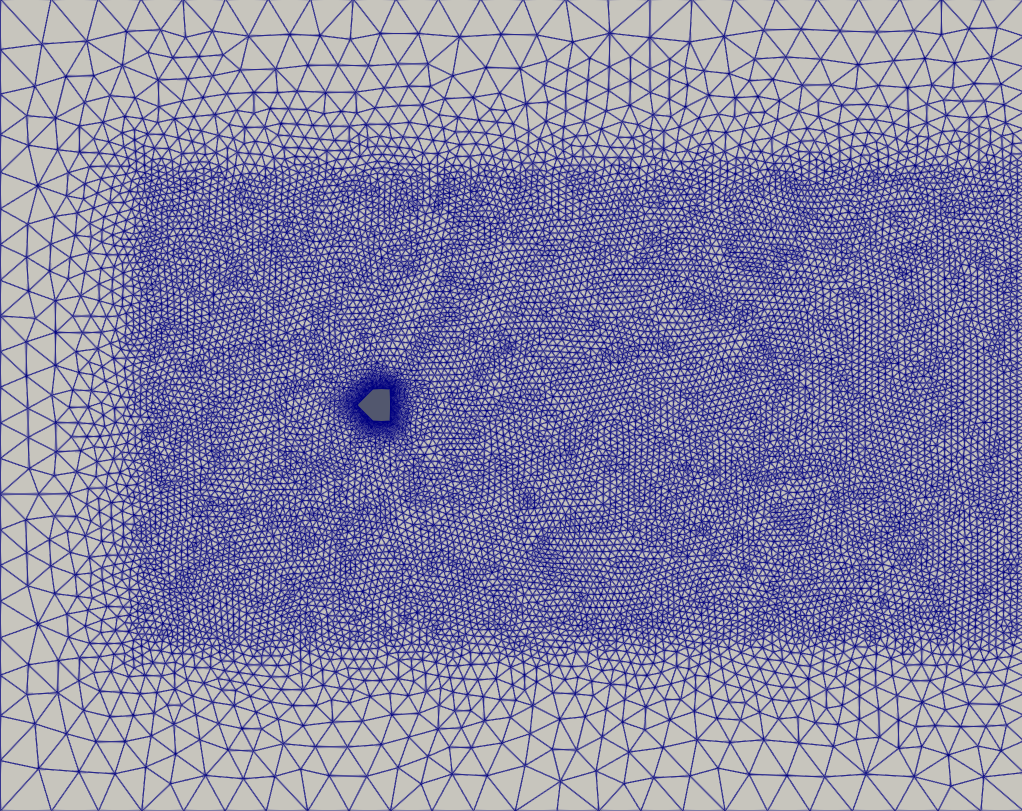
\includegraphics[width=\textwidth]{images/2FaceMesh}
	\caption{Example of mesh of fluid domain with bluff body $n = 2$. Visualized in ParaView}
	\label{fig:2FaceMesh}
\end{figure}

\subsubsection{The OpenFOAM Simulation}
\label{sec:openFoam}
The theoretical part of this EE was conducted using the open-source CFD software package OpenFOAM \parencite{noauthor_openfoam_2024} in Windows Subsystem for Linux (WSL) \parencite{noauthor_windows_nodate}. Among the numerous solvers OpenFOAM provides, pimpleFOAM is a transient, pressure-based solver for incompressible, single-phase flows \parencite{noauthor_pimplefoam_nodate}. It facilitates robust handling of transient simulations with larger time steps, allowing for improved computational performance. Moreover, its ability to model both laminar and turbulent flow ensures flow conditions are accurately reflected and given that the fluctuations of lift force in laminar flow are sinusoidal, one can verify the flow is laminar. Utilizing reporting functions, one can extract the lift coefficient $C_{L}$, which shows the fluctuations in the lift force acting on the bluff body.
\subsubsection{Simulation Settings}
\label{sec:simulationSettings}
To adhere to the scope of this essay, the simulation setup was adapted from a case study provided in the Udemy course \textit{OpenFOAM for Absolute Beginners} by \textcite{jayaraj2024openfoam}. The tutorial case \textit{3vortexShedding}, discussed in lecture eight, served as a structural template and was modified to align with the specific requirements of this investigation.

\vspace{1em}

\begin{figure}[H]
	\centering
	\begin{forest}
		for tree={
			font=\ttfamily,
			grow=east,
			child anchor=west,
			parent anchor=east,
			anchor=west,
			edge={draw,-stealth},
			inner sep=2pt,
			l sep=50pt,
			s sep=20pt
		}
		[case/
		[0/
		[\textcolor{blue}{U}]
		[p]
		[nuTilda]
		[nut]
		]
		[constant/
		[turbulenceProperties]
		[\textcolor{blue}{transportProperties}]
		[g]
		[\textcolor{green}{polyMesh/}
		[\textcolor{green}{pointZones}]
		[\textcolor{green}{points}]
		[\textcolor{green}{owner}]
		[\textcolor{green}{neighbor}]
		[\textcolor{green}{faceZones}]
		[\textcolor{green}{faces}]
		[\textcolor{green}{cellZones}]
		[\textcolor{green}{boundary}]
		]
		]
		[system/
		[fvSolution]
		[fvSchemes]
		[\textcolor{green}{forceCoeffs}]
		[\textcolor{blue}{decomposeParDict}]
		[\textcolor{blue}{controlDict}]
		]
		[\textcolor{blue}{para.foam}]
		[\textcolor{blue}{mesh.msh}]
		]
	\end{forest}
	\caption{Overview of the simulation directory structure. Modified files are highlighted blue. Created files and folders are highlighted green }
\end{figure}


\begin{table}[H]
	\centering
	\makebox[\linewidth][c]{
		\begin{tabularx}{1.2\textwidth}{|p{3cm}|p{3.3cm}|p{2.8cm}|p{3cm}|X|}
			\hline
			\textbf{File} & \textbf{Parameter} & \textbf{Original} & \textbf{Modified} & \textbf{Justification} \\
			\hline
			\verb*|mesh.msh|, \verb*|para.foam|, 
			\begin{tabular}[t]{@{}l@{}}
				\verb|polyMesh/|\\[-0.3em]
				\small\hspace{1.5em}\verb|boundary| \\[-0.3em]
				\small\hspace{1.5em}\verb|cellZones| \\[-0.3em]
				\small\hspace{1.5em}\verb|faces| \\[-0.3em]
				\small\hspace{1.5em}\verb|faceZones| \\[-0.3em]
				\small\hspace{1.5em}\verb|neighbor| \\[-0.3em]
				\small\hspace{1.5em}\verb|owner| \\[-0.3em]
				\small\hspace{1.5em}\verb|points| \\[-0.3em]
				\small\hspace{1.5em}\verb|pointsZones|
			\end{tabular} 
			
			& \textemdash & \verb*|mesh.msh| defines, \verb*|polyMesh/| contains and \verb*|para.foam| visualizes the mesh of fluid domain of tutorial case & \verb*|mesh.msh| defines, \verb*|polyMesh/| contains and \verb*|para.foam| visualizes the mesh of fluid domain with dimensions given in \Cref{sec:ansysWorkbench} & The fluid domain was adjusted to conform with the computational limits discussed in \Cref{sec:ansysWorkbench}, while achieving the Reynolds number required for this investigation\\
			\hline
			\verb*|controlDict| & \verb*|deltaT| & 0.0002 & 0.00001 &
			Decreased in order to achieve a greater accuracy \parencite[289]{versteeg2007} while ensuring numerical stability \parencite{caminha_cfl_2017}. 
			\\
			
			\rule{0pt}{5ex} & \verb*|functions| & \verb*|none| &
			\begin{tabular}[t]{@{}l@{}}
				\verb|#include| \\[-0.3em]
				\verb*|"forceCoeffs"|
			\end{tabular} &
			Reporting function, defined in \verb*|forceCoeffs|, included in order to extract the lift coefficient $C_L$ \parencite{codeynamics_prism_2024}
			\\ 
			
			\rule{0pt}{5ex} & {\small\verb*|adjustTimeStep|} & \verb*|yes| & \verb*|no| &
			Removed as the simulation demonstrated stable behavior with the adjusted \verb*|deltaT| \parencite{jayaraj2024openfoam}
			\\ 
			
			\hline
			
			
		\end{tabularx}
	}
	\caption{Overview of the changes made to the simulation template.}
	\label{tab:simulation_change1}
\end{table}

\begin{table}[H]
	\centering
	\renewcommand{\arraystretch}{1.3}
	\makebox[\linewidth][c]{
		\begin{tabularx}{1.2\textwidth}{|p{3cm}|p{3.3cm}|p{2.8cm}|p{3cm}|X|}
			\hline
			\textbf{File} & \textbf{Parameter} & \textbf{Original} & \textbf{Modified} & \textbf{Justification} \\
			\hline
			
			{\footnotesize\verb*|decomposeParDict|} & {\footnotesize\verb*|numberOfSubdomains|} & 8 & 6 & The simulations were performed on a system with \verb*|6| processing cores \parencite{jayaraj2024openfoam} \\
			\hline
			
			\verb*|forceCoeffs| & \textemdash & \textemdash & Created a reporting function which outputs the variation of the lift coefficient $C_L$ throughout the simulation & Lift coefficient $C_L$ is needed for subsequent calculation of vortex shedding frequency $f$\\
			\hline
			
			{\scriptsize\verb*|transportProperties|} & \verb*|nu| & \SI{1e5}{} & \SI{1e6}{} & The kinematic viscosity of water at 20\si{\celsius} is approximately \SI{1e6}{\meter\squared\per\second} \parencite{noauthor_water_nodate}\\
			\hline
			\verb*|U|& \texttt{inlet value} \newline \texttt{(x, y, z)} & x = \num{10} & x = \num{0.1} & Adapted in order to achieve the target Reynolds number of \num{100} using \Cref{eq:reynoldsNumber} where $L=\SI{1e-3}{\meter}$, $\nu = \SI{1e-6}{\meter\squared\per\second}$ and $U = \SI{0.1}{\meter\per\second}$ \\
			\hline
		\end{tabularx}
	}
	\caption*{\textbf{Table 3 (continued):} Overview of the changes made to the simulation template.}
	\label{tab:simulation_changes2}
	
\end{table}




\subsection{The Practical Investigation}
\label{sec:practicalMethod}

\begin{figure}[H]
	\centering
	\begin{tikzpicture}
		\path[use as bounding box] (-8, -7) rectangle (10, 7);
		\node[inner sep=0pt] (img) at (0,0) {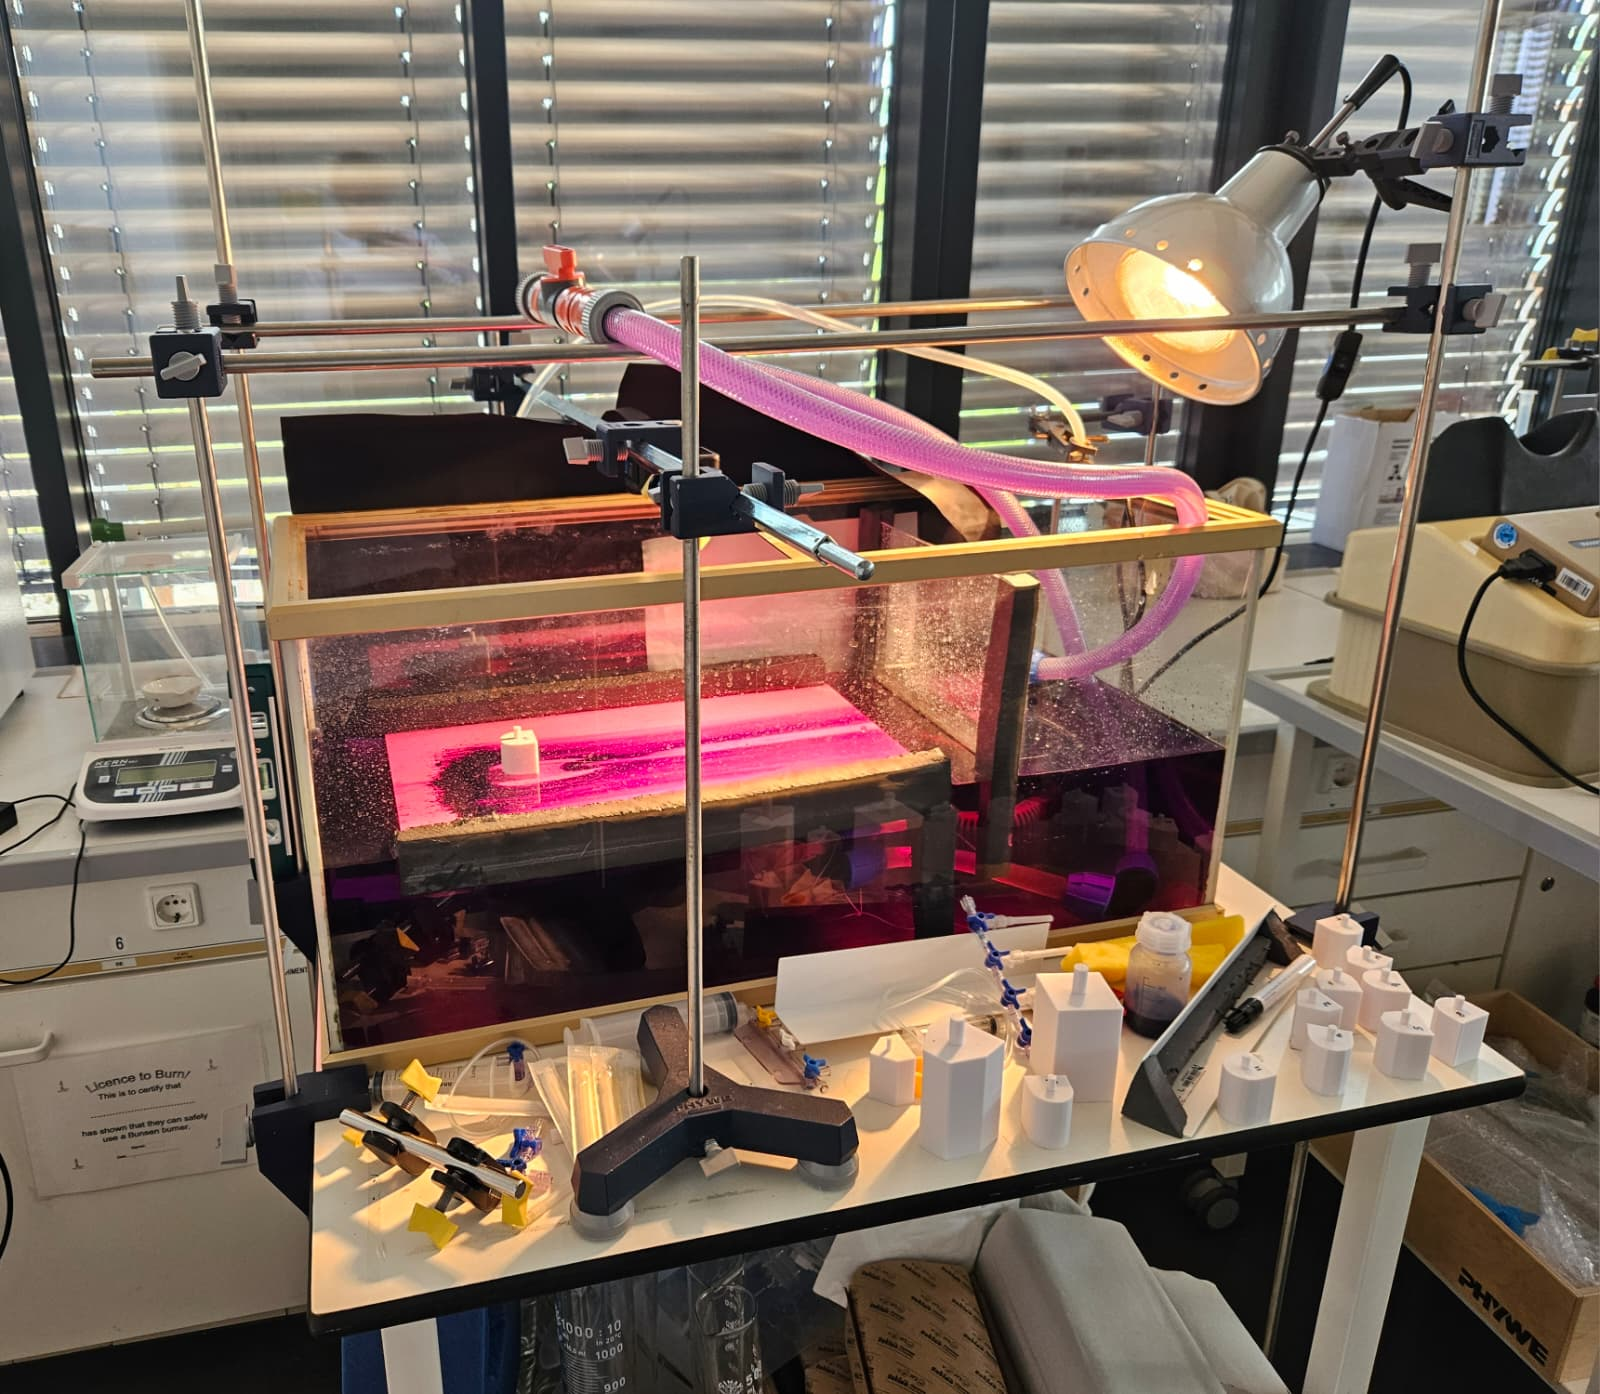
\includegraphics[width=\textwidth]{images/overallSetup1.jpg}};
		
		
		%Right
		\draw[->, line width=2pt, color=red] (6.5, 4.5) -- (4.2, 4.2);
		\node[draw, fill=white, line width=1pt, anchor=west] at (6.6, 4.5) {Lamp};
		
		\draw[->, line width=2pt, color=red] (6.5, 3.25) -- (2, 3.3);
		\node[draw, fill=white, line width=1pt, anchor=west, align=left] at (6.6, 3.25) {Hose (water \\[-0.6em] supply)};
		
		\draw[->, line width=2pt, color=red] (6.5, 2) -- (2.9, 2.5);
		\node[draw, fill=white, line width=1pt, anchor=west] at (6.6, 2) {Clamp};
		
		\draw[->, line width=2pt, color=red] (6.5, 0) -- (3.9, 1);
		\node[draw, fill=white, line width=1pt, anchor=west] at (6.6, 0) {Piping \diameter \SI{0.017}{\meter}};
		
		\draw[->, line width=2pt, color=red] (6.5, -1) -- (2, -0.2);
		\node[draw, fill=white, line width=1pt, anchor=west, align=left] at (6.6, -1) {Separation wall (2)};
		
		\draw[->, line width=2pt, color=red] (6.5, -2) -- (1.35, -1.6);
		\node[draw, fill=white, line width=1pt, anchor=west, align=left] at (6.6, -2) {Separation wall (1)};
		
		\draw[->, line width=2pt, color=red] (6.5, -4) -- (0.1, -1.8);
		\node[draw, fill=white, line width=1pt, anchor=west, align=left] at (6.6, -4) {Sponge diffuser};
		
		% Left
		\draw[->, line width=2pt, color=red] (-6.5, -2) -- (-5, 0);
		\node[draw, fill=white, line width=1pt, anchor=east, align=left] at (-6.6, -2) {Aquarium};
		
		
	\end{tikzpicture}
	\caption{The setup for the practical investigation (angle 1)}
	\label{fig:overallSetup1}
\end{figure}

\begin{figure}[H]
	\centering
	\begin{tikzpicture}
		\path[use as bounding box] (-8, -7.5) rectangle (10, 7);
		
		\node[inner sep=0pt] (img) at (0,0) {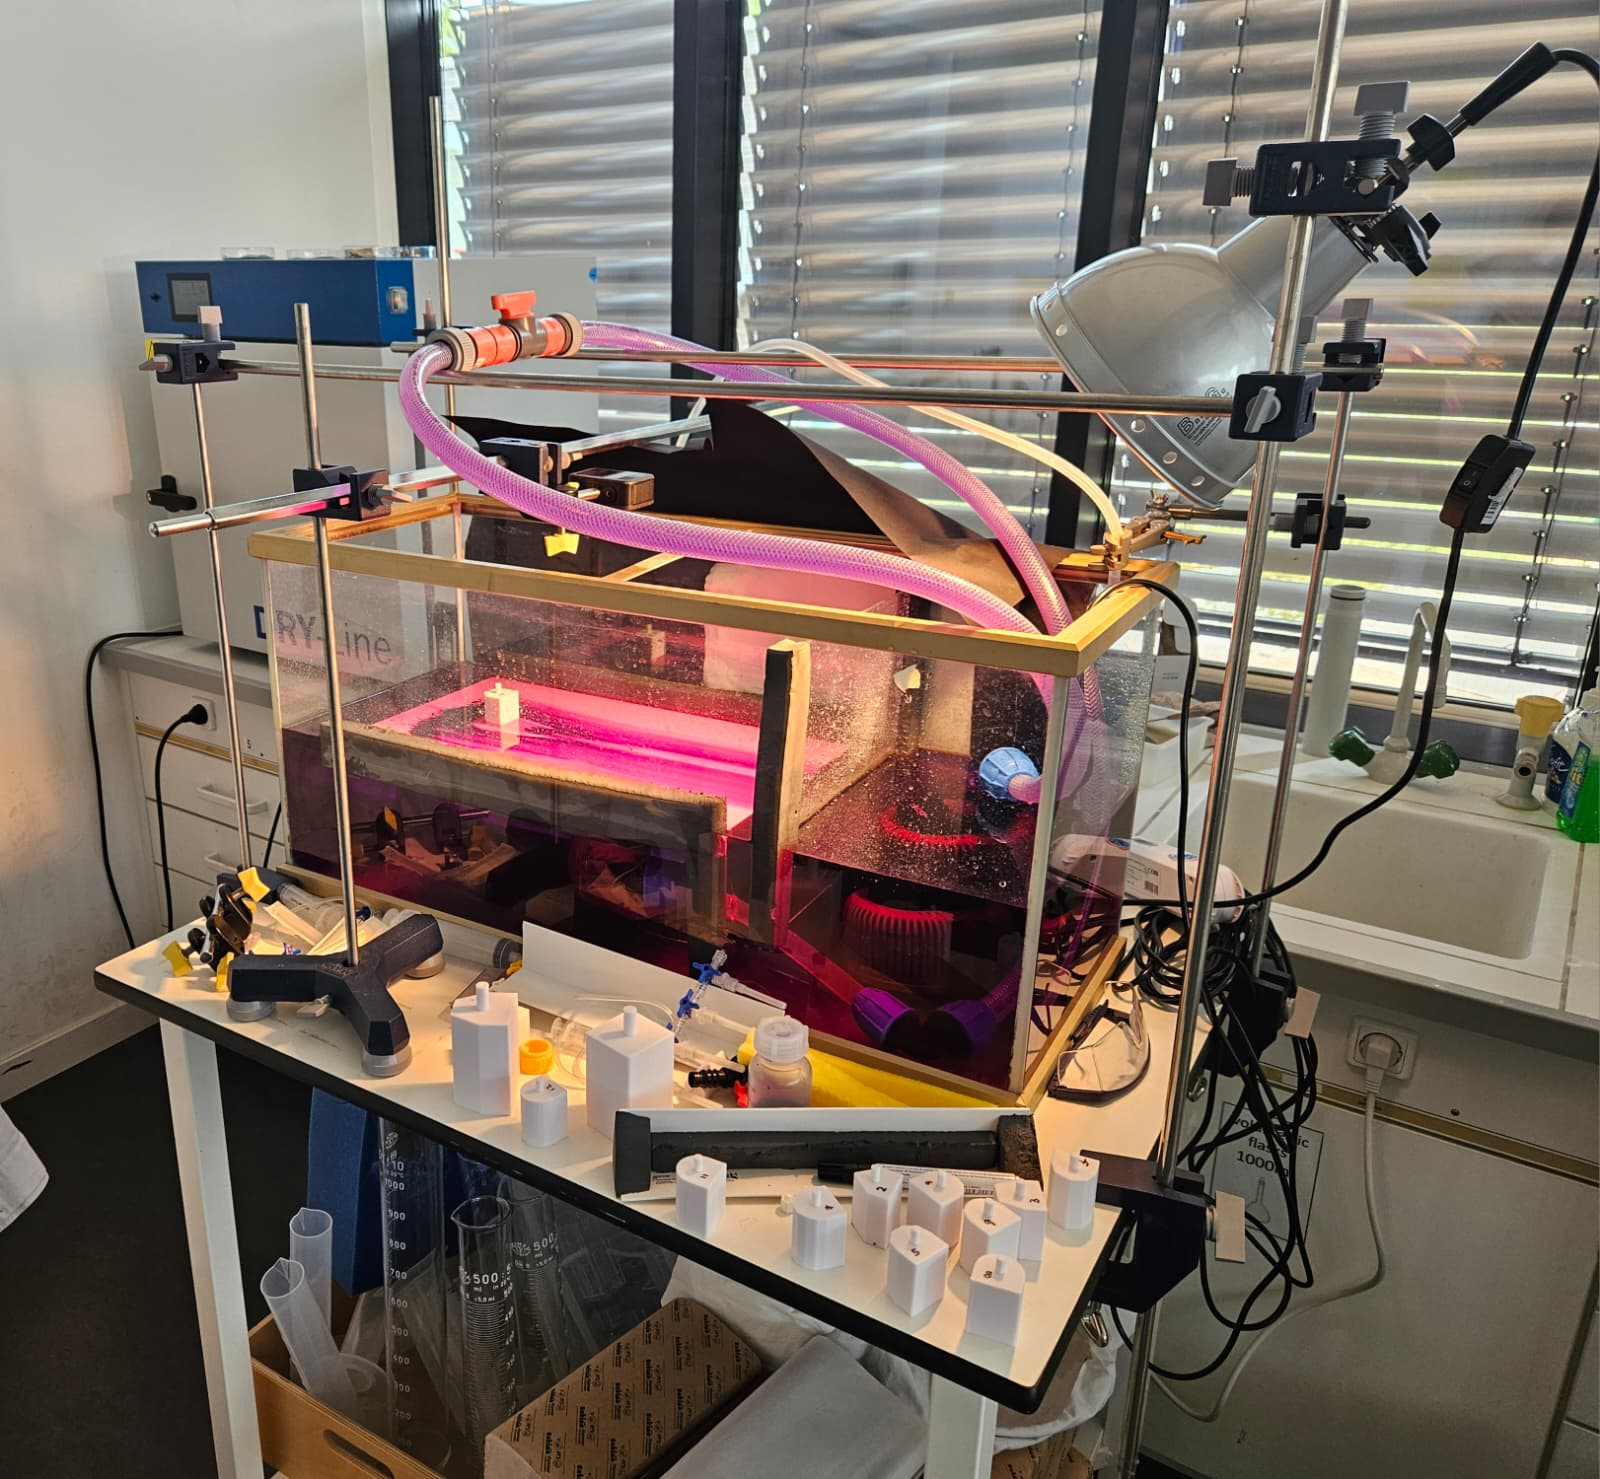
\includegraphics[width=\textwidth]{images/overallSetup2.jpg}};
		
		% Right
		\draw[->, line width=2pt, color=red] (6.5, 2) -- (4.9, 3.3);
		\node[draw, fill=white, line width=1pt, anchor=west] at (6.6, 2) {Boss};
		
		\draw[->, line width=2pt, color=red] (6.5, 0) -- (4.4, 1);
		\node[draw, fill=white, line width=1pt, anchor=west] at (6.6, 0) {Metal rod};
		
		\draw[->, line width=2pt, color=red] (6.5, -1) -- (0.4, 0);
		\node[draw, fill=white, line width=1pt, anchor=west] at (6.6, -1) {Clear acrylic glass};
		
		\draw[->, line width=2pt, color=red] (6.5, -2) -- (1.3, -2);
		\node[draw, fill=white, line width=1pt, anchor=west, align=left] at (6.6, -2) {\SI{75}{\watt} Water pump};
		
		\draw[->, line width=2pt, color=red] (6.5, -3) -- (1.5, -3);
		\node[draw, fill=white, line width=1pt, anchor=west, align=left] at (6.6, -3) {Pipe corner piece};
		
		\draw[->, line width=2pt, color=red] (6.5, -4) -- (3.8, -4.6);
		\node[draw, fill=white, line width=1pt, anchor=west, align=left] at (6.6, -4) {Screw clamp};
		
		% Left
		\draw[->, line width=2pt, color=red] (-6.5, -4) -- (-5, -2.5);
		\node[draw, fill=white, line width=1pt, anchor=east, align=left] at (-6.6, -4) {Table stand};
		
		\draw[->, line width=2pt, color=red] (-6.5, 1) -- (-2, 2.5);
		\node[draw, fill=white, line width=1pt, anchor=east, align=left] at (-6.6, 1) {GoPro};
		
		\draw[->, line width=2pt, color=red] (-6.5, 4) -- (-3, 4);
		\node[draw, fill=white, line width=1pt, anchor=east, align=left] at (-6.6, 4) {Regulation value};
		
		
		
		
	\end{tikzpicture}
	\caption{The setup for the practical investigation (angle 2)}
	\label{fig:overallSetup2}
\end{figure}

\begin{figure}[H]
	\centering
	\begin{tikzpicture}
		\node[inner sep=0pt] at (0,0) {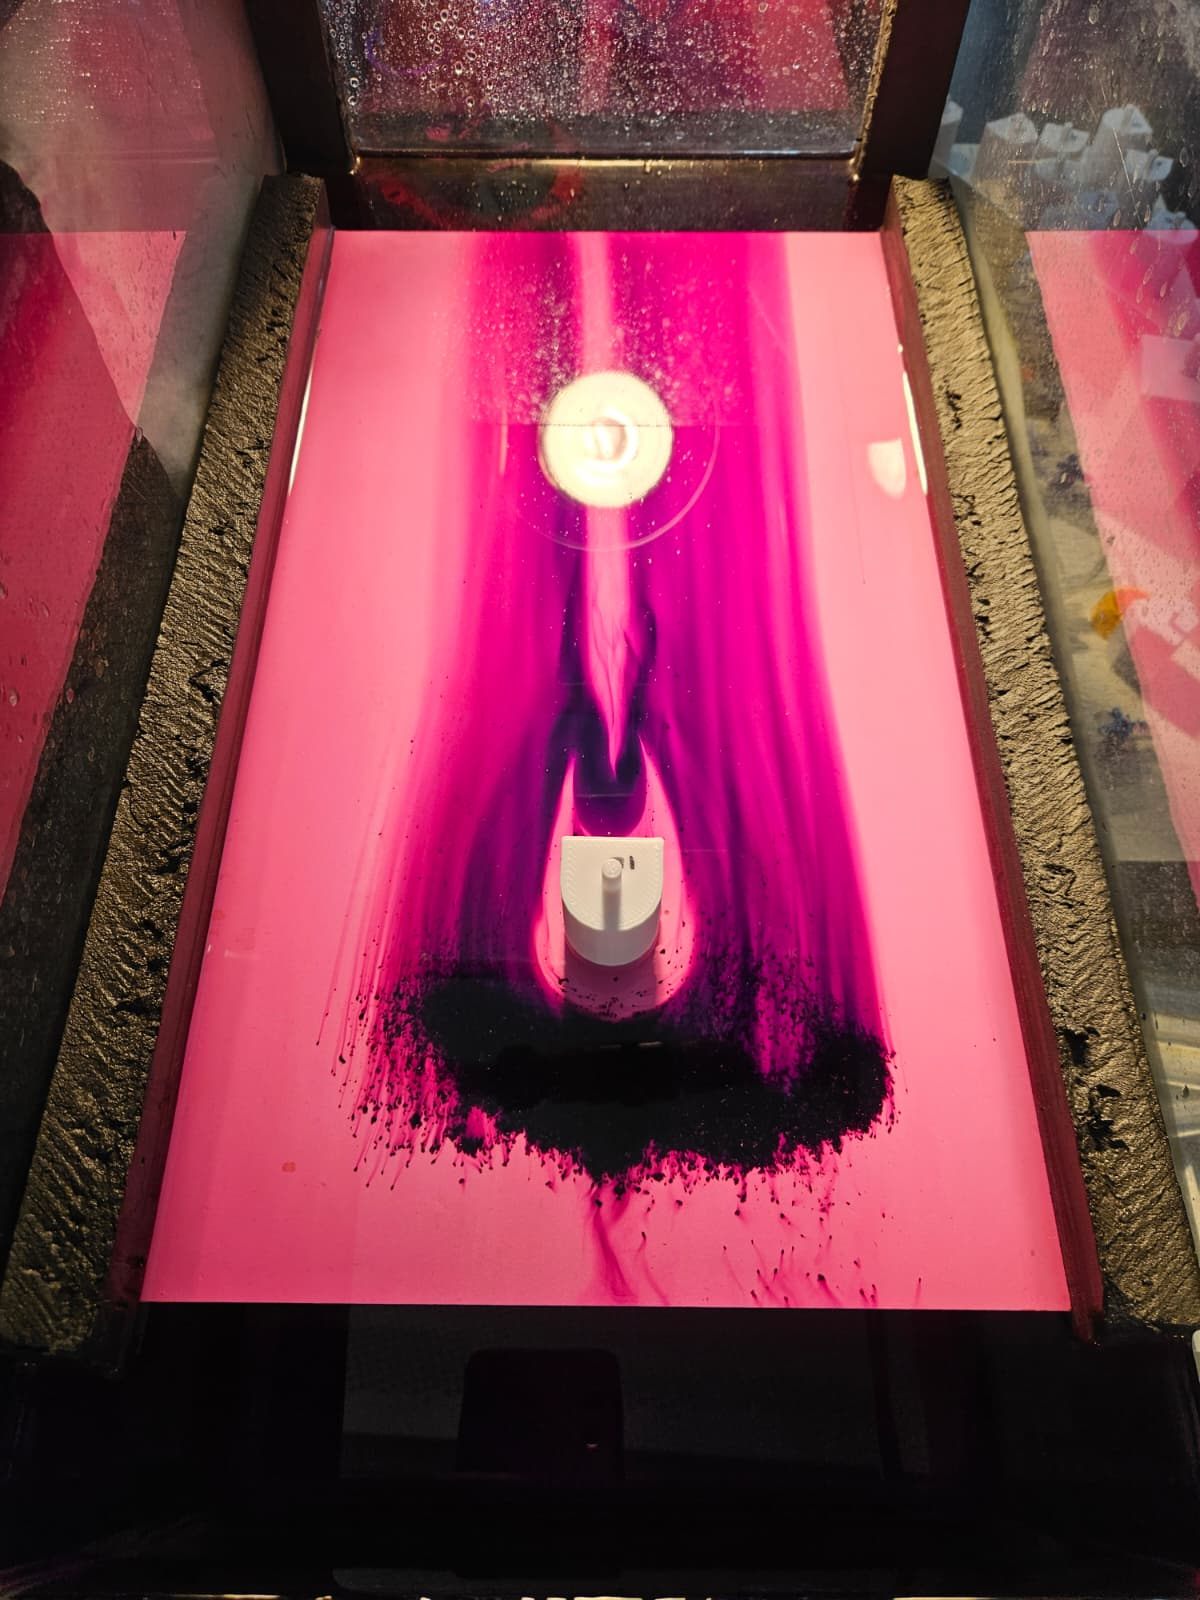
\includegraphics[width=\textwidth]{images/shapeInTank.jpg}};
		
		% Left
		\draw[->, line width=2pt, color=red] (6.5, 4.5) -- (5, 4.2);
		\node[draw, fill=white, line width=1pt, anchor=west, align=left] at (6.6, 4.5) {Thermal insulation \\[-0.6em] foam};
		
		\draw[->, line width=2pt, color=red] (6.5, 2) -- (3.7, 2.5);
		\node[draw, fill=white, line width=1pt, anchor=west] at (6.6, 2) {White acrylic glass};
		
		\draw[->, line width=2pt, color=red] (6.5, -1) -- (0.9, -2);
		\node[draw, fill=white, line width=1pt, anchor=west, align=left] at (6.6, -1) {Reference Mark};
		
		\draw[->, line width=2pt, color=red] (6.5, -4) -- (0.8, -4);
		\node[draw, fill=white, line width=1pt, anchor=west, align=left] at (6.6, -4) {Potassium \\[-0.6em] permanganate \\[-0.6em] crystals};
		
		
		
		
	\end{tikzpicture}
	\caption{A bluff body positioned in the flow tank with potassium permanganate crystals spread in front of it}
	\label{fig:shapeInTank}
\end{figure}

\begin{figure}[H]
	\centering
	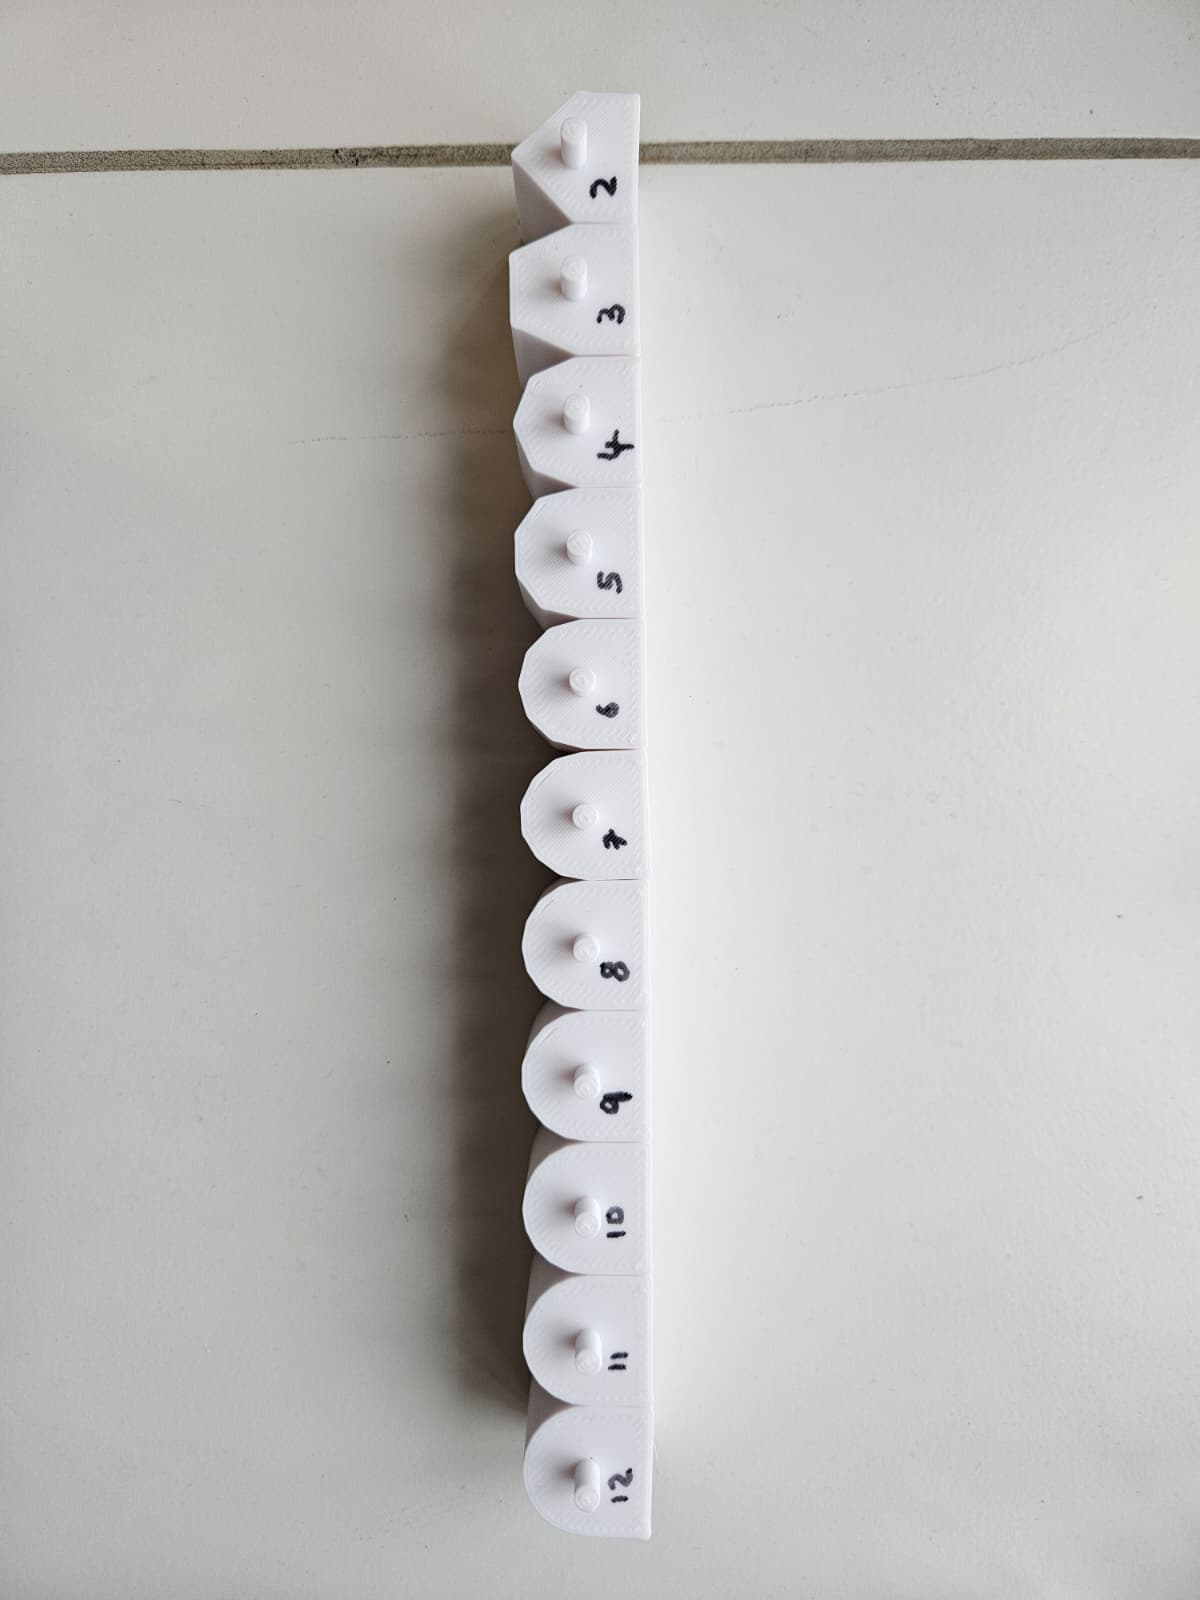
\includegraphics[width=\textwidth]{images/shapes.jpg}
	\caption{The 3D-printed bluff bodies. The numbers correspond to the number of inlet-facing sides}
	\label{fig:shapes}
\end{figure}

\newpage

Inspired by the flow tank built by Harvard University’s Science Demonstrations Center \parencite{noauthor_vortex_nodate}, the practical part of this EE was conducted in a self-built flow tank. A water pump created a flow over a horizontal plate by moving water from one side of separation wall (1) to the other. Separation wall (2), which did not reach the bottom of the tank, forced the flow of the horizontal wall towards the pump. The aquarium was filled with water so that it reached \SI{0.01}{\meter} above the horizontal plate. The regulation valve was used to decrease the flow velocity while the sponge diffuser ensured a uniform distribution of flow \textemdash\ in an attempt to achieve laminar flow. Both a lamp and the addition of potassium permanganate crystals in front of the shape were used in order to better visualize the water flow. The thermal insulation foam ensured watertightness between the aquarium wall and the inside components. 

The bluff bodies were 3D printed with an overall length $\ell$ of \SI{0.02}{\meter} \textemdash\ giving each shape a characteristic length $L$ of \SI{0.02}{\meter} \textemdash\ and a height of \SI{0.04}{\meter}. Pre-tests showed that this overall length proved to be the optimal balance between the size of the bluff bodies and adequate identification of produced vortices, in an attempt to achieve a Reynolds number of \num{100}. Reference marks on the horizontal plate ensured the shape was positioned consistently each trial. A GoPro recording in 120 FPS was mounted parallel to the horizontal plate, ensuring a continuous recording of the entire horizontal plate. The outer scaffolding provided support for the lamp, the GoPro and the water supply hose. 

The flow velocity for the subsequent calculation of the Reynolds number was measured using a basic time-distance method, wherein a float was introduced and the time taken to travel the length of the horizontal plate was measured via a digital stopwatch. This was repeated ten times and an average was taken.

\subsection{Determining the vortex shedding frequency}
The inverse relationship given by \Cref{eq:fAndT} in section \Cref{sec:fAndT} will be used to determine the vortex shedding frequency. By measuring the time interval between the formation of two consecutive vertices on one side of the bluff body, one can find the time period and therefore the frequency of vortex shedding. To obtain an accurate vortex shedding frequency, the determination of the time period was completed after periodic vortex shedding was achieved, omitting the initial startup phase in which the flow developed. A Fast Fourier Transform approach was not chosen due to the lack of sufficient runtime during the trials on either investigation and the absence of multiple different frequencies of vortex shedding \parencites[10--11]{shi2025vortex}[12]{xu_experimental_2025}.

\subsubsection{Theoretical Investigation}
\label{sec:theoreticalMethod}
The simulation was run five times for each bluff body. It was found that each iteration of a bluff body yielded the same results, therefore only the first run of each bluff body was considered. By graphing fluctuations of the lift coefficient \textemdash\ as can be seen in \Cref{sec:C_LvsTime} \textemdash\ one can calculate the time period of vortex shedding by identifying the time taken between two consecutive peaks or troughs. This determination was done for each peak and trough using Python \textemdash\ see Listing~A.\ref{lst:freqDetermination} \textemdash\ removing the first second to omit the startup phase. An average time period was then calculated and the vortex shedding frequency was found. ParaView was used to visualize the simulation.

\subsubsection{Practical Investigation}
The bluff bodies were placed into the flow tank at the position of the reference marks. Wearing gloves and goggles, minimal amounts of potassium permanganate were placed in front of them using a spatula \textemdash\ as shown in \Cref{fig:shapeInTank}. Once the flow fully developed, it was recorded for one minute each time. This minimized the number of water replacements \textemdash\ due to dissolving potassium permanganate turning the water purple \textemdash\ while ensuring that one could take multiple measurements of the time period. The water was reused for four shapes before the aquarium was emptied using a hand pump \textemdash\ disposing the solution in a properly assigned waste tank \textemdash\ and was refilled with fresh water. 

The time period of vortex shedding was found via visual inspection of the GoPro footage and using a digital stop watch. It was repeated ten times for each bluff body. An average was subsequently calculated and the vortex shedding frequency was determined.

\section{Results}
\subsection{Results of the Theoretical Investigation}

\subsubsection{Sample Tables of Time vs. Lift Coefficient ($C_L$) for Bluff Body $n=2,\,6\,\text{and}\,12$}

\begin{table}[H]
	\centering
	\renewcommand{\arraystretch}{1.3}
	\begin{tabular}{|c|c|}
		\hline
		\textbf{Time (s)} & \textbf{$C_L$} \\
		\hline
		$1 \times 10^{-5}$ & $2.0946206 \times 10^{-11}$ \\
		$2 \times 10^{-5}$ & $-6.5426717 \times 10^{-12}$ \\
		$3 \times 10^{-5}$ & $-7.3241302 \times 10^{-12}$ \\
		$4 \times 10^{-5}$ & $-6.6677951 \times 10^{-12}$ \\
		$5 \times 10^{-5}$ & $-5.1304516 \times 10^{-12}$ \\
		$6 \times 10^{-5}$ & $-4.3635501 \times 10^{-12}$ \\
		$7 \times 10^{-5}$ & $-3.6837751 \times 10^{-12}$ \\
		$8 \times 10^{-5}$ & $-3.2635206 \times 10^{-12}$ \\
		$9 \times 10^{-5}$ & $-2.8660898 \times 10^{-12}$ \\
		$1.0 \times 10^{-4}$ & $-2.4321206 \times 10^{-12}$ \\
		$1.1 \times 10^{-4}$ & $-2.1246574 \times 10^{-12}$ \\
		$1.2 \times 10^{-4}$ & $-1.8807166 \times 10^{-12}$ \\
		$1.3 \times 10^{-4}$ & $-1.6461582 \times 10^{-12}$ \\
		$1.4 \times 10^{-4}$ & $-1.4100222 \times 10^{-12}$ \\
		$1.5 \times 10^{-4}$ & $-1.1994923 \times 10^{-12}$ \\
		$1.6 \times 10^{-4}$ & $-1.0306274 \times 10^{-12}$ \\
		$1.7 \times 10^{-4}$ & $-8.6746456 \times 10^{-13}$ \\
		$1.8 \times 10^{-4}$ & $-7.3730846 \times 10^{-13}$ \\
		$1.9 \times 10^{-4}$ & $-6.2413158 \times 10^{-13}$ \\
		$2.0 \times 10^{-4}$ & $-5.1195718 \times 10^{-13}$ \\
		$2.1 \times 10^{-4}$ & $-4.1747569 \times 10^{-13}$ \\
		$2.2 \times 10^{-4}$ & $-3.2864061 \times 10^{-13}$ \\
		$2.3 \times 10^{-4}$ & $-2.6866516 \times 10^{-13}$ \\
		$2.4 \times 10^{-4}$ & $-2.1575370 \times 10^{-13}$ \\
		$2.5 \times 10^{-4}$ & $-1.7389840 \times 10^{-13}$ \\
		\hline
	\end{tabular}
	\label{tab:1FaceClTable}
	\caption{Example of the first 25 values of the table produced by the simulation. Time vs. Lift Coefficient ($C_L$) for bluff body $n=2$}
\end{table}

\begin{table}[H]
	\centering
	\renewcommand{\arraystretch}{1.3}
	\begin{tabular}{|c|c|}
		\hline
		\textbf{Time (s)} & \textbf{$C_L$} \\
		\hline
		$1 \times 10^{-5}$  & $-3.3657419 \times 10^{-12}$ \\
		$2 \times 10^{-5}$  & $-1.9884762 \times 10^{-11}$ \\
		$3 \times 10^{-5}$  & $-9.3048242 \times 10^{-12}$ \\
		$4 \times 10^{-5}$  & $-4.4630770 \times 10^{-12}$ \\
		$5 \times 10^{-5}$  & $-2.0927449 \times 10^{-12}$ \\
		$6 \times 10^{-5}$  & $-7.7780466 \times 10^{-13}$ \\
		$7 \times 10^{-5}$  & $-6.0321899 \times 10^{-14}$ \\
		$8 \times 10^{-5}$  & $4.8061350 \times 10^{-13}$ \\
		$9 \times 10^{-5}$  & $7.3193765 \times 10^{-13}$ \\
		$1.0 \times 10^{-4}$ & $9.6907823 \times 10^{-13}$ \\
		$1.1 \times 10^{-4}$ & $1.1376576 \times 10^{-12}$ \\
		$1.2 \times 10^{-4}$ & $1.2174253 \times 10^{-12}$ \\
		$1.3 \times 10^{-4}$ & $1.2584116 \times 10^{-12}$ \\
		$1.4 \times 10^{-4}$ & $1.3129809 \times 10^{-12}$ \\
		$1.5 \times 10^{-4}$ & $1.3234668 \times 10^{-12}$ \\
		$1.6 \times 10^{-4}$ & $1.3258472 \times 10^{-12}$ \\
		$1.7 \times 10^{-4}$ & $1.3305942 \times 10^{-12}$ \\
		$1.8 \times 10^{-4}$ & $1.3123542 \times 10^{-12}$ \\
		$1.9 \times 10^{-4}$ & $1.2928728 \times 10^{-12}$ \\
		$2.0 \times 10^{-4}$ & $1.2666382 \times 10^{-12}$ \\
		$2.1 \times 10^{-4}$ & $1.2276206 \times 10^{-12}$ \\
		$2.2 \times 10^{-4}$ & $1.1975532 \times 10^{-12}$ \\
		$2.3 \times 10^{-4}$ & $1.1559278 \times 10^{-12}$ \\
		$2.4 \times 10^{-4}$ & $1.1103320 \times 10^{-12}$ \\
		$2.5 \times 10^{-4}$ & $1.0755046 \times 10^{-12}$ \\
		\hline
	\end{tabular}
	\label{tab:6FaceClTable}
	\caption{Example of the first 25 values of the table produced by the simulation. Time vs. Lift Coefficient ($C_L$) for bluff body $n=6$}
\end{table}

\begin{table}[H]
	\centering
	\renewcommand{\arraystretch}{1.3}
	\begin{tabular}{|c|c|}
		\hline
		\textbf{Time (s)} & \textbf{$C_L$} \\
		\hline
		$1 \times 10^{-5}$  & $-2.4598505 \times 10^{-11}$ \\
		$2 \times 10^{-5}$  & $7.6579451 \times 10^{-12}$ \\
		$3 \times 10^{-5}$  & $-2.1510813 \times 10^{-12}$ \\
		$4 \times 10^{-5}$  & $-4.4206937 \times 10^{-12}$ \\
		$5 \times 10^{-5}$  & $-2.2353308 \times 10^{-12}$ \\
		$6 \times 10^{-5}$  & $-3.6197725 \times 10^{-12}$ \\
		$7 \times 10^{-5}$  & $-2.8919916 \times 10^{-12}$ \\
		$8 \times 10^{-5}$  & $-2.1972666 \times 10^{-12}$ \\
		$9 \times 10^{-5}$  & $-1.6629472 \times 10^{-12}$ \\
		$1.0 \times 10^{-4}$ & $-1.1636706 \times 10^{-12}$ \\
		$1.1 \times 10^{-4}$ & $-7.5429574 \times 10^{-13}$ \\
		$1.2 \times 10^{-4}$ & $-4.0834742 \times 10^{-13}$ \\
		$1.3 \times 10^{-4}$ & $-1.3927346 \times 10^{-13}$ \\
		$1.4 \times 10^{-4}$ & $2.5593892 \times 10^{-13}$ \\
		$1.5 \times 10^{-4}$ & $4.2789616 \times 10^{-13}$ \\
		$1.6 \times 10^{-4}$ & $6.3422462 \times 10^{-13}$ \\
		$1.7 \times 10^{-4}$ & $5.5145736 \times 10^{-13}$ \\
		$1.8 \times 10^{-4}$ & $6.3739292 \times 10^{-13}$ \\
		$1.9 \times 10^{-4}$ & $6.7691966 \times 10^{-13}$ \\
		$2.0 \times 10^{-4}$ & $7.1047796 \times 10^{-13}$ \\
		$2.1 \times 10^{-4}$ & $7.3849782 \times 10^{-13}$ \\
		$2.2 \times 10^{-4}$ & $7.3959605 \times 10^{-13}$ \\
		$2.3 \times 10^{-4}$ & $7.3249622 \times 10^{-13}$ \\
		$2.4 \times 10^{-4}$ & $7.3044772 \times 10^{-13}$ \\
		$2.5 \times 10^{-4}$ & $7.3234202 \times 10^{-13}$ \\
		\hline
	\end{tabular}
	\label{tab:12FaceClTable}
	\caption{Example of the first 30 values of the table produced by the simulation. Time vs. Lift Coefficient ($C_L$) for bluff body $n=12$}
\end{table}

\subsubsection{Lift Coefficient ($C_L$) Over Time for each Bluff Body}

\begin{figure}[H]
	\centering
	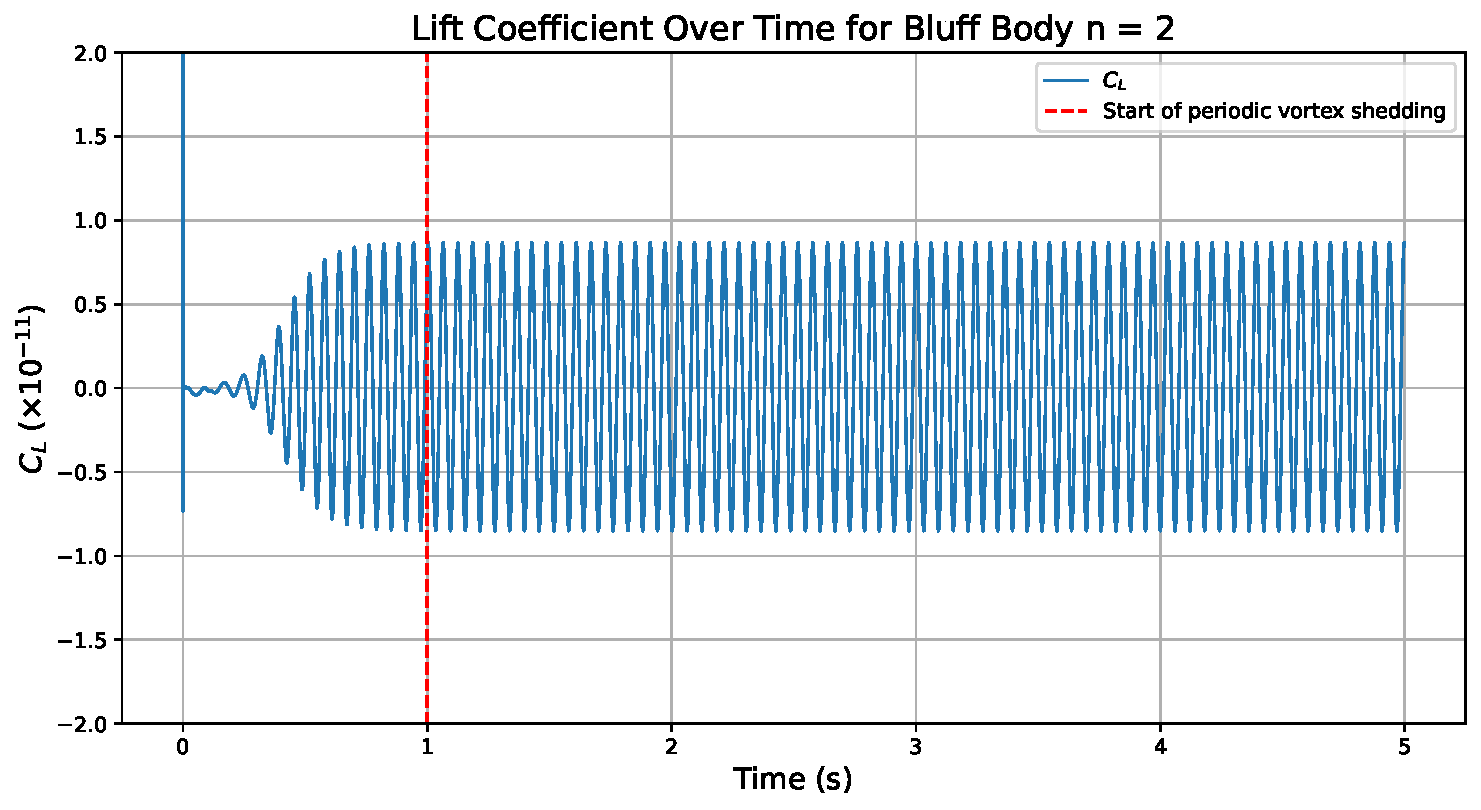
\includegraphics[width=\textwidth]{images/2face_graph}
	\caption{Lift coefficient $C_L$ over time for the bluff body $n=2$. The red dashed line indicates the start of the steady-state phase at $t = 1\,\mathrm{s}$.}
	\label{fig:2FaceGraph}
\end{figure}

\begin{figure}[H]
	\centering
	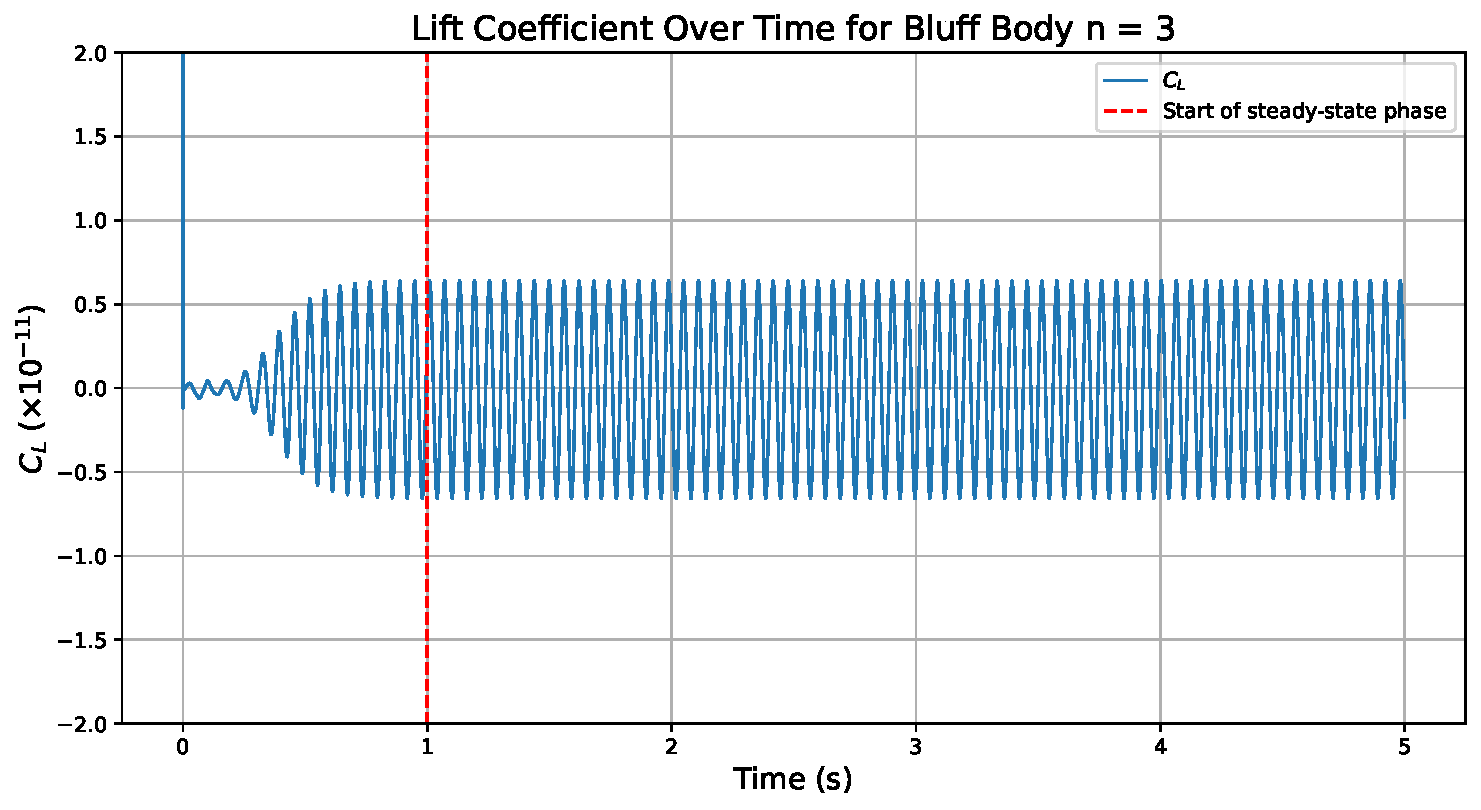
\includegraphics[width=\textwidth]{images/3face_graph}
	\caption{Lift coefficient $C_L$ over time for the bluff body $n=3$. The red dashed line indicates the start of the steady-state phase at $t = 1\,\mathrm{s}$.}
	\label{fig:3FaceGraph} 
\end{figure}

\begin{figure}[H]
	\centering
	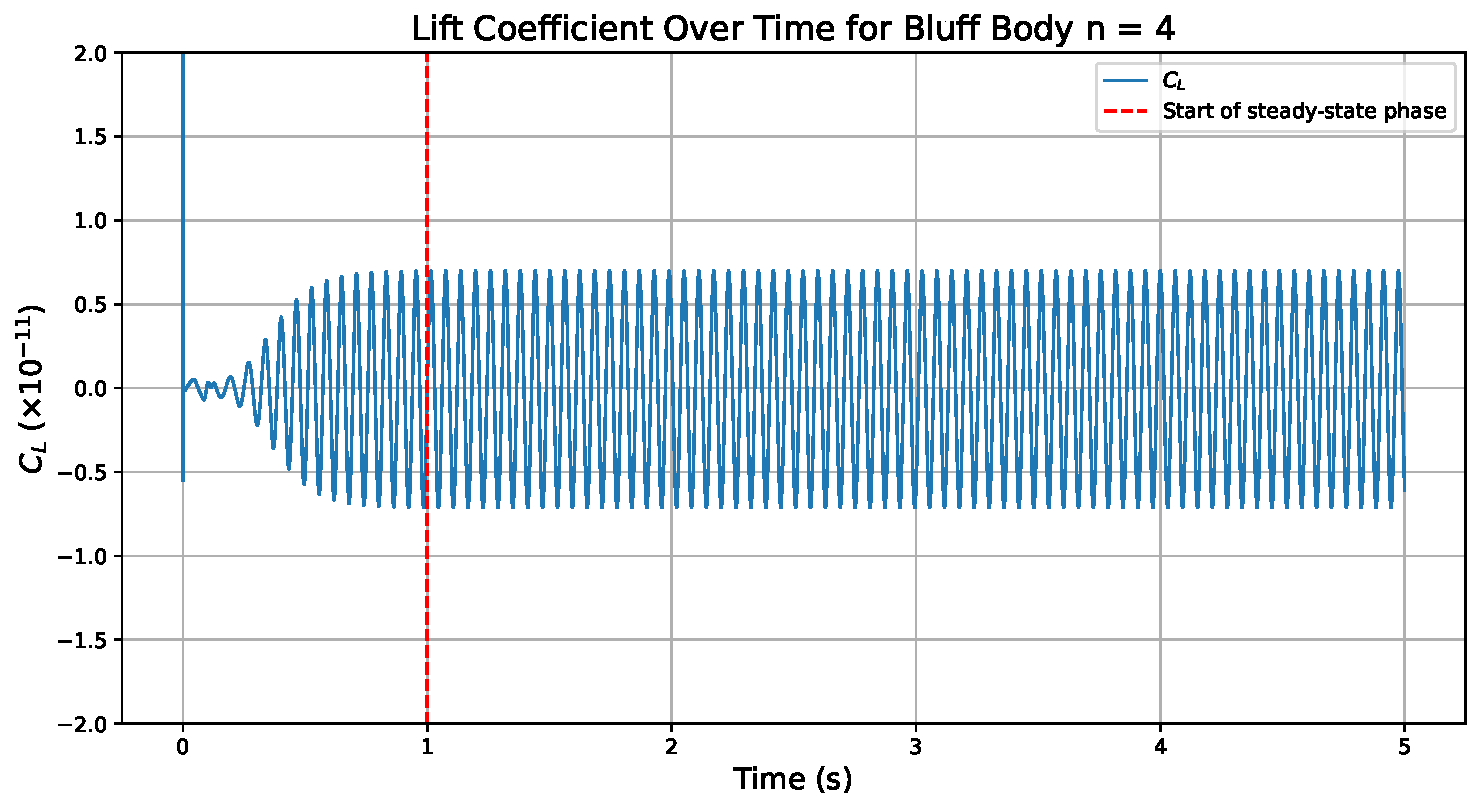
\includegraphics[width=\textwidth]{images/4face_graph}
	\caption{Lift coefficient $C_L$ over time for the bluff body $n=4$. The red dashed line indicates the start of the steady-state phase at $t = 1\,\mathrm{s}$.}
	\label{fig:4FaceGraph} 
\end{figure}

\begin{figure}[H]
	\centering
	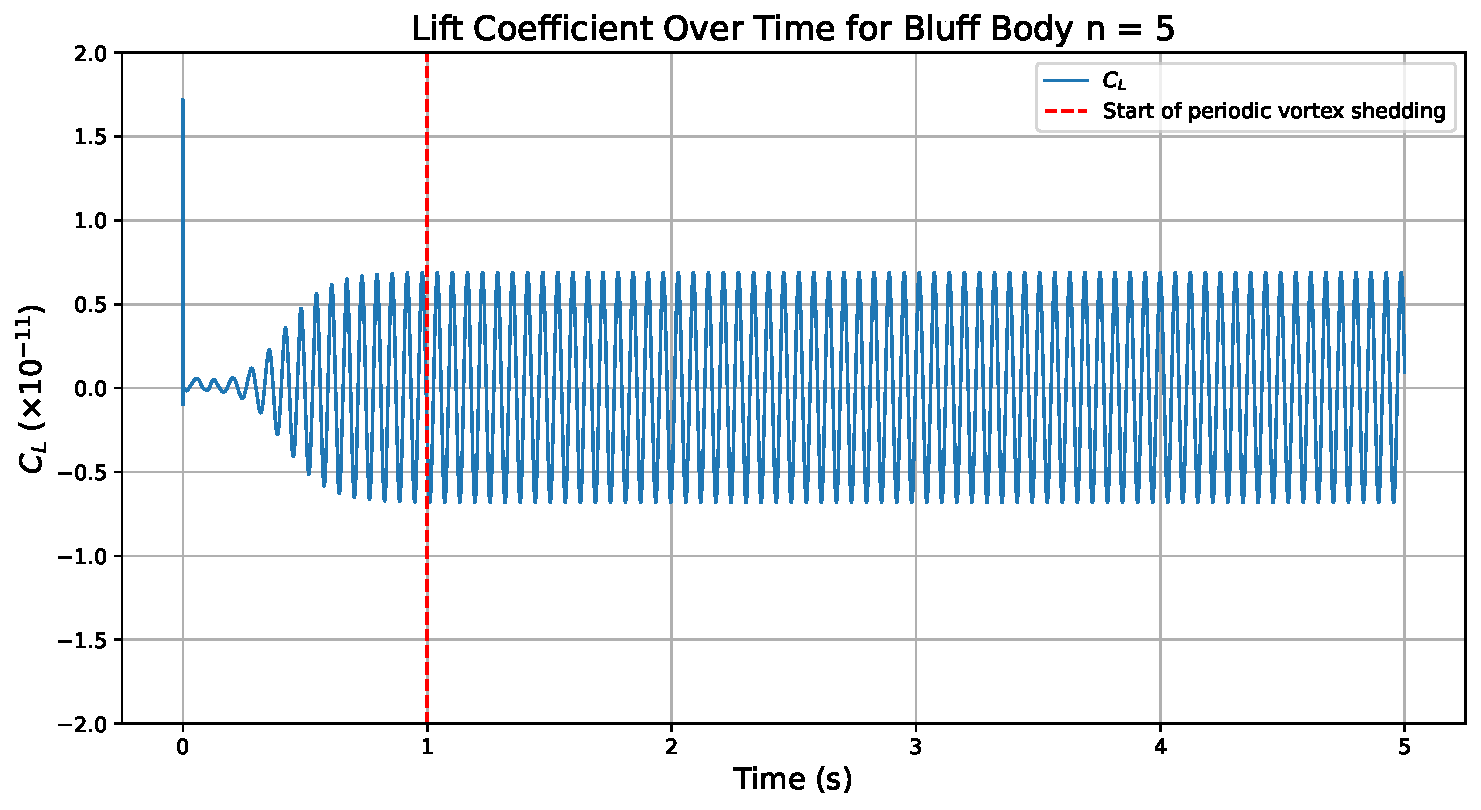
\includegraphics[width=\textwidth]{images/5face_graph}
	\caption{Lift coefficient $C_L$ over time for the bluff body $n=5$. The red dashed line indicates the start of the steady-state phase at $t = 1\,\mathrm{s}$.}
	\label{fig:5FaceGraph} 
\end{figure}

\begin{figure}[H]
	\centering
	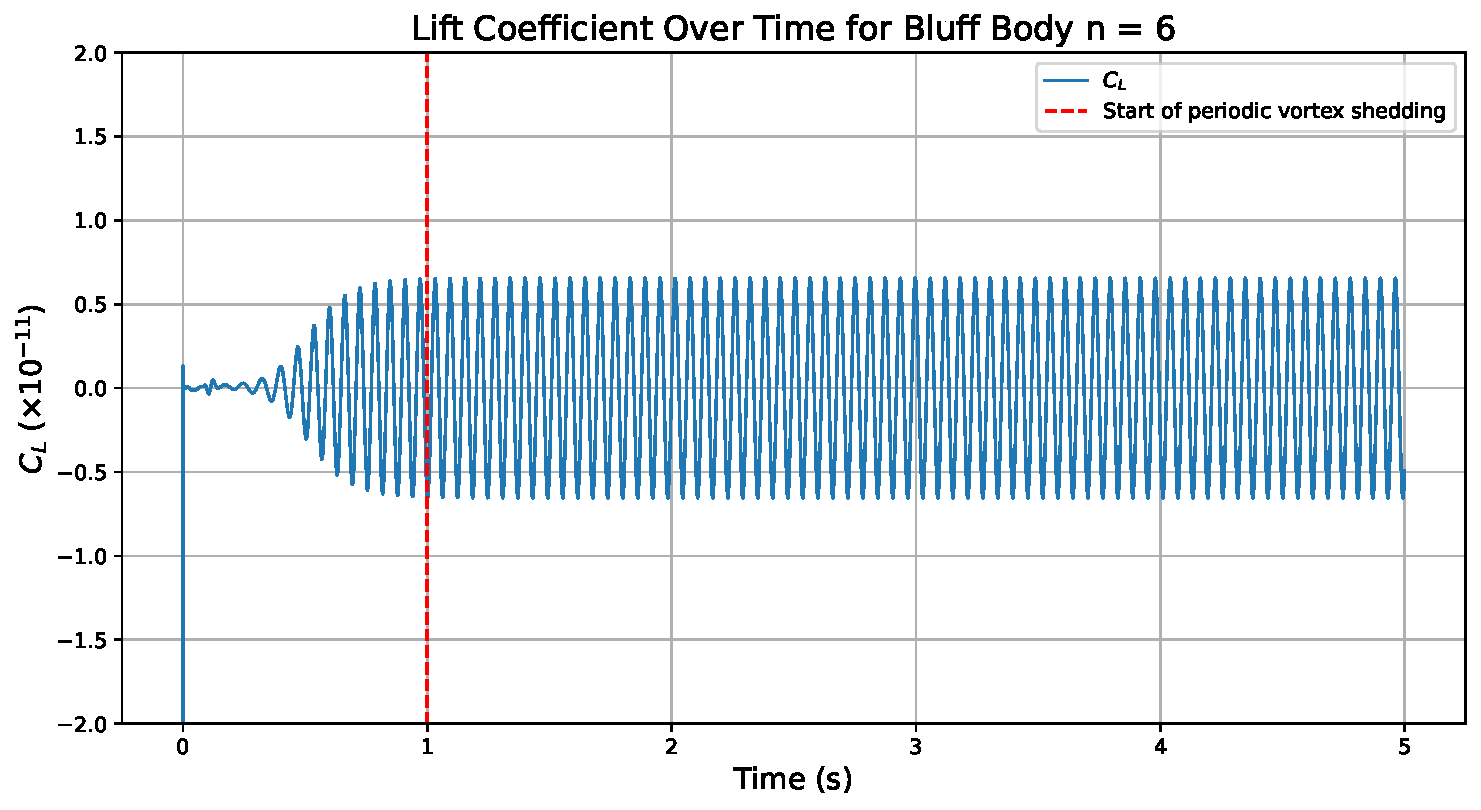
\includegraphics[width=\textwidth]{images/6face_graph}
	\caption{Lift coefficient $C_L$ over time for the bluff body $n=6$. The red dashed line indicates the start of the steady-state phase at $t = 1\,\mathrm{s}$.}
	\label{fig:6FaceGraph} 
\end{figure}

\begin{figure}[H]
	\centering
	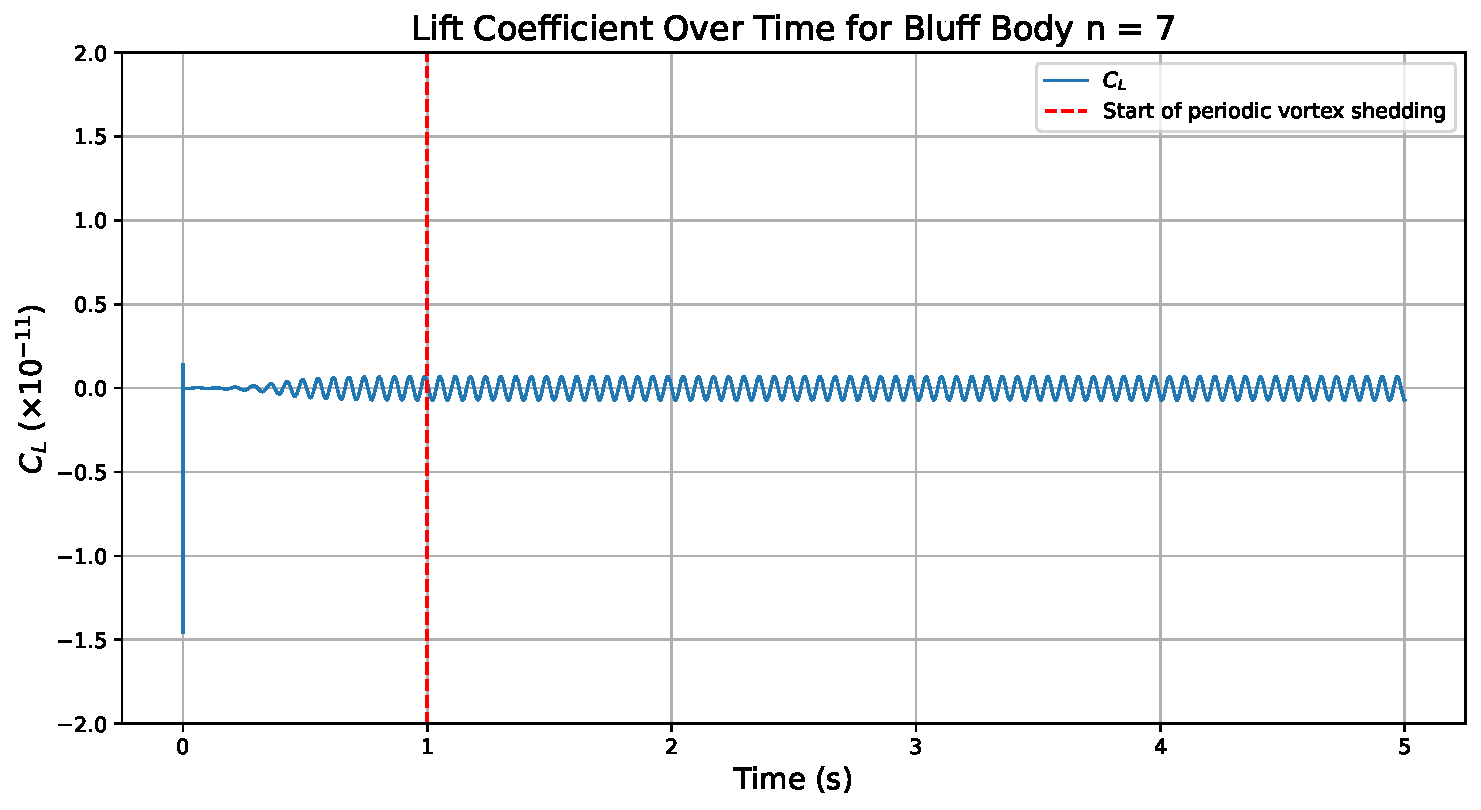
\includegraphics[width=\textwidth]{images/7face_graph}
	\caption{Lift coefficient $C_L$ over time for the bluff body $n=7$. The red dashed line indicates the start of the steady-state phase at $t = 1\,\mathrm{s}$.}
	\label{fig:7FaceGraph} 
\end{figure}

\begin{figure}[H]
	\centering
	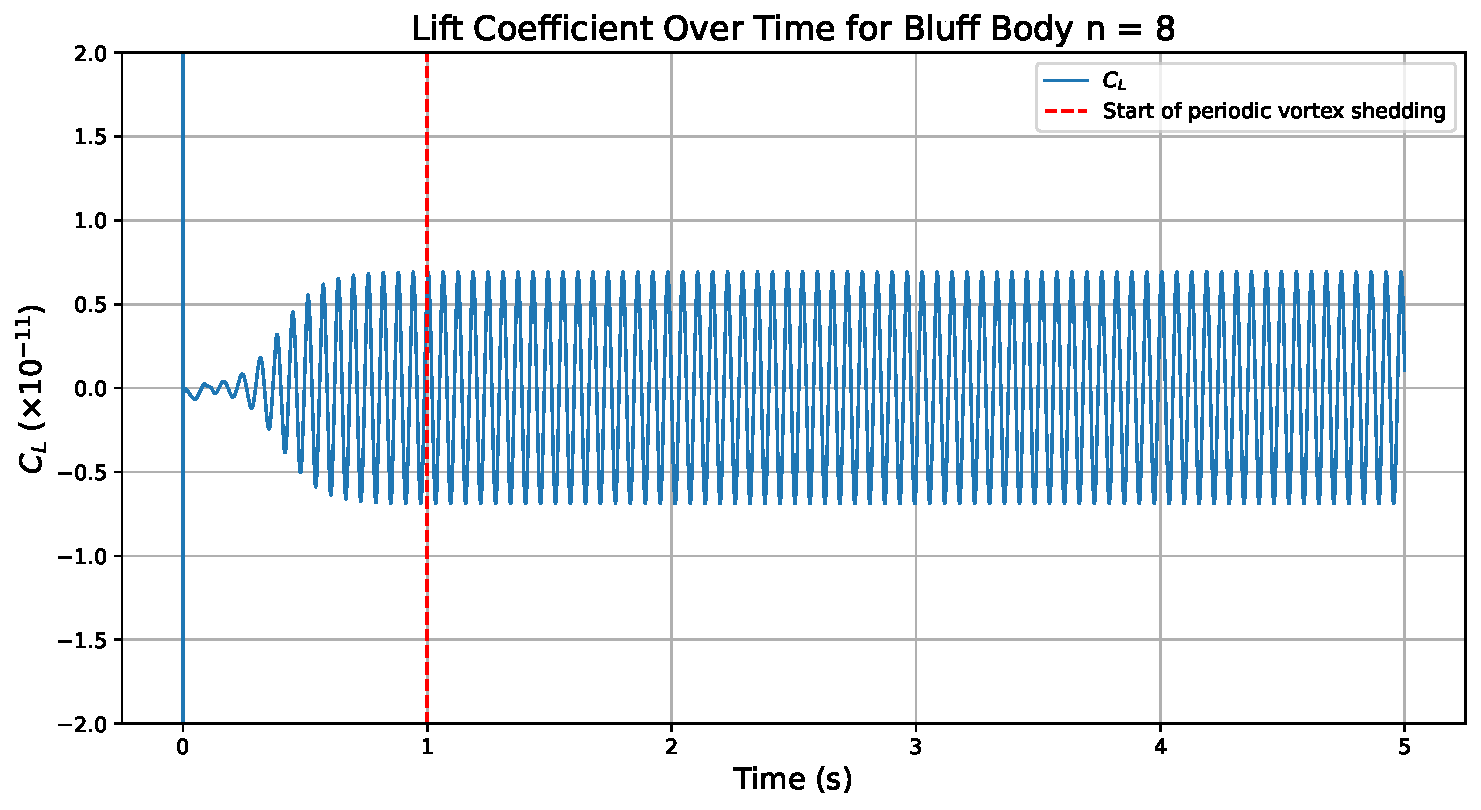
\includegraphics[width=\textwidth]{images/8face_graph}
	\caption{Lift coefficient $C_L$ over time for the bluff body $n=8$. The red dashed line indicates the start of the steady-state phase at $t = 1\,\mathrm{s}$.}
	\label{fig:8FaceGraph} 
\end{figure}

\begin{figure}[H]
	\centering
	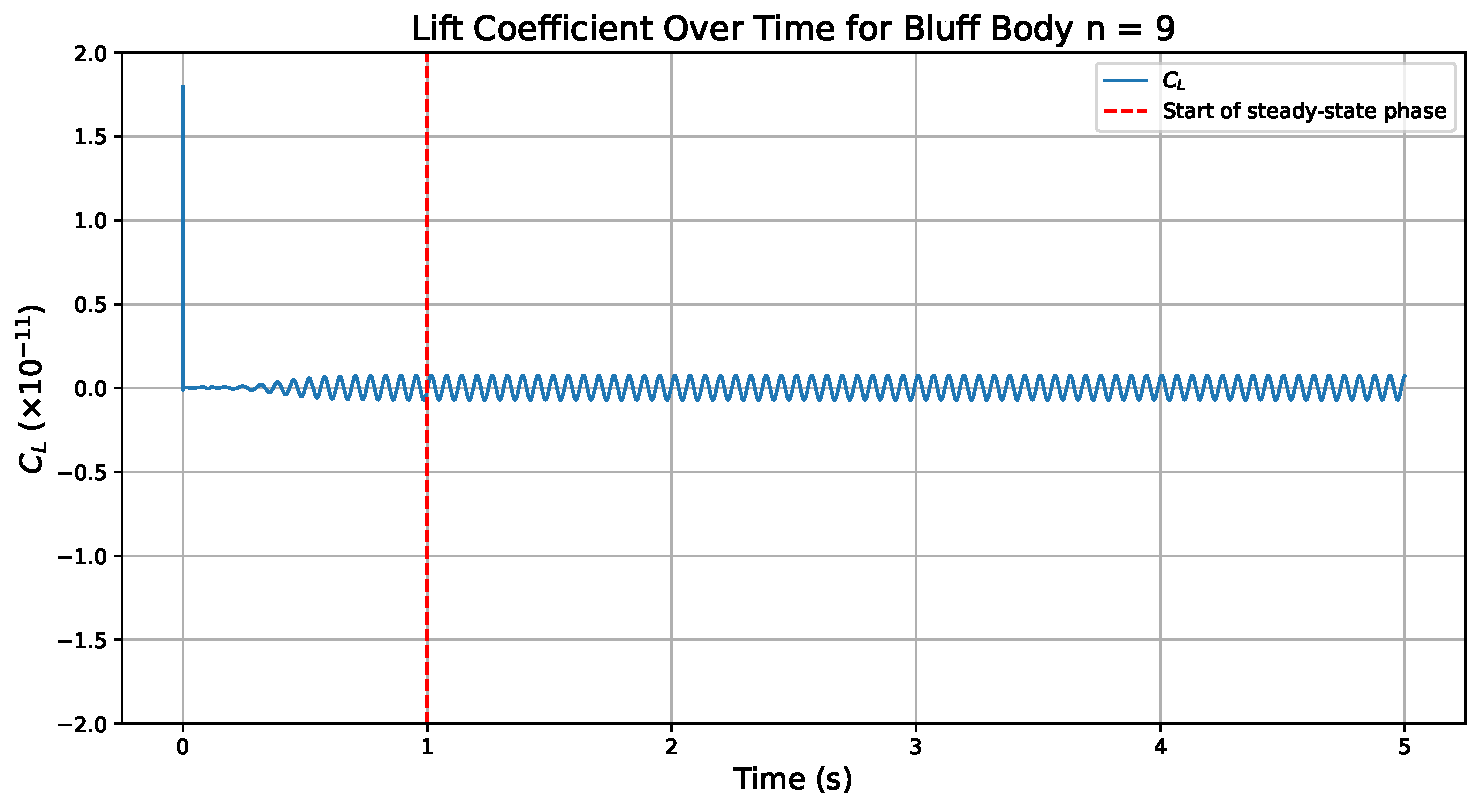
\includegraphics[width=\textwidth]{images/9face_graph}
	\caption{Lift coefficient $C_L$ over time for the bluff body $n=9$. The red dashed line indicates the start of the steady-state phase at $t = 1\,\mathrm{s}$.}
	\label{fig:9FaceGraph} 
\end{figure}

\begin{figure}[H]
	\centering
	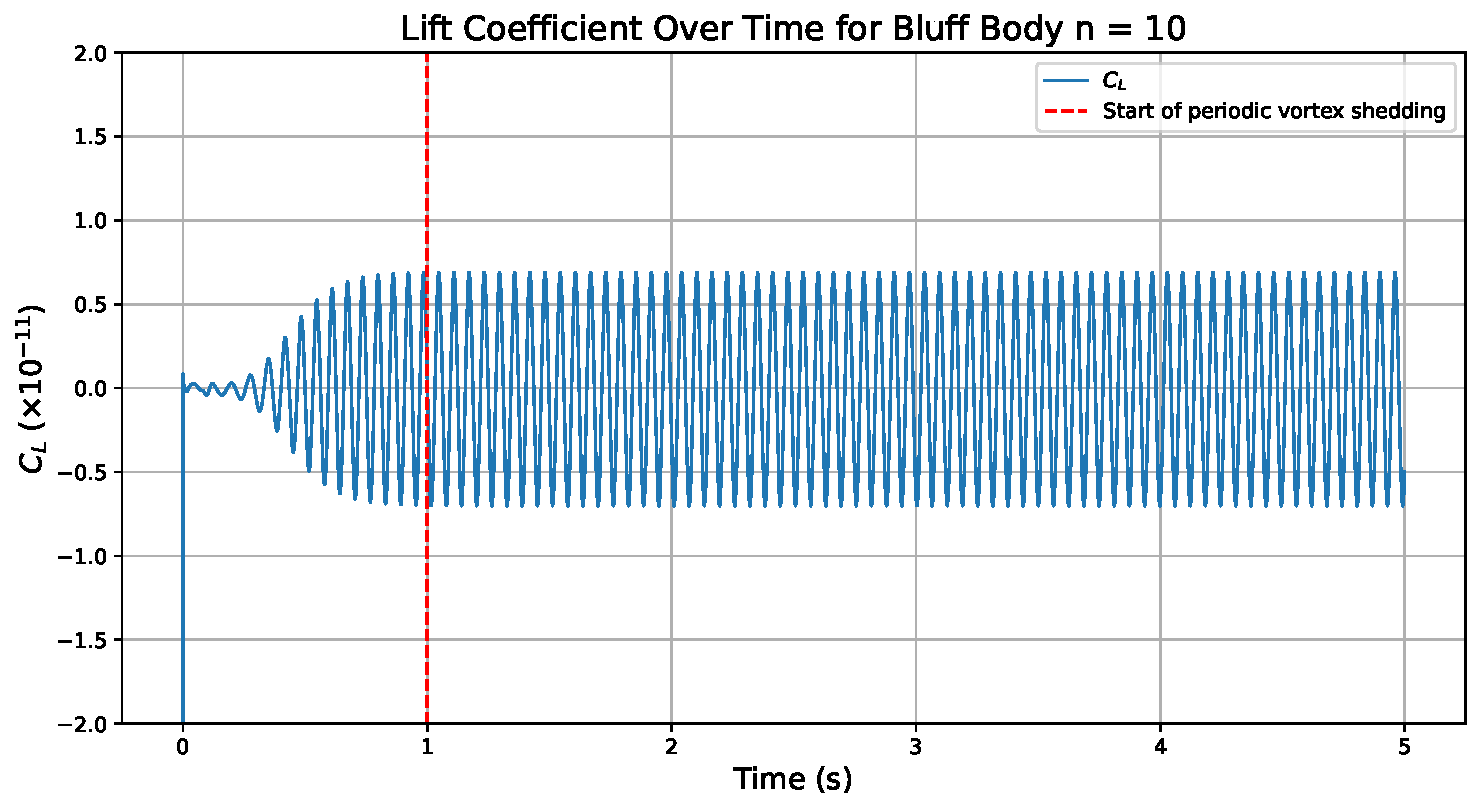
\includegraphics[width=\textwidth]{images/10face_graph}
	\caption{Lift coefficient $C_L$ over time for the bluff body $n=10$. The red dashed line indicates the start of the steady-state phase at $t = 1\,\mathrm{s}$.}
	\label{fig:10FaceGraph} 
\end{figure}

\begin{figure}[H]
	\centering
	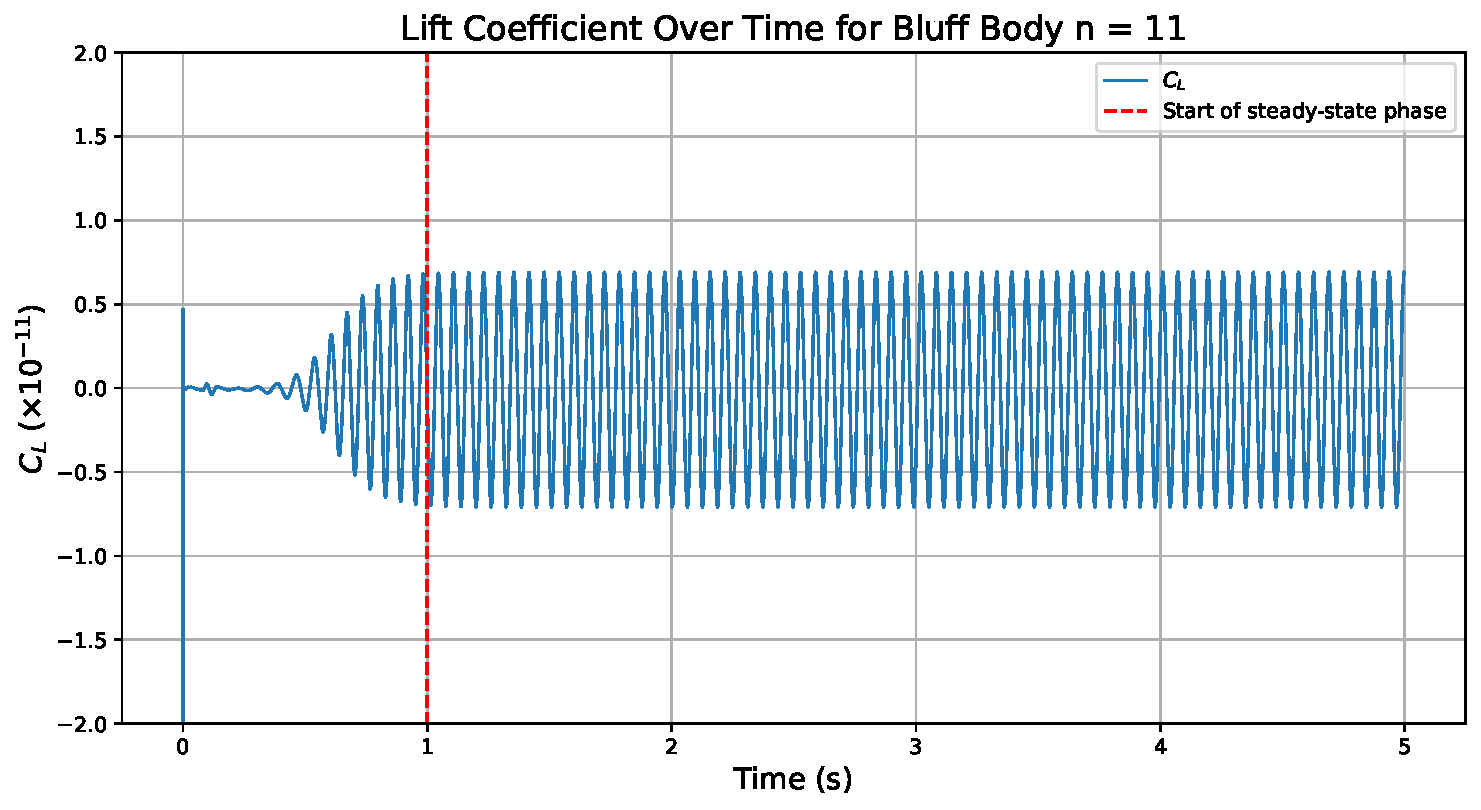
\includegraphics[width=\textwidth]{images/11face_graph}
	\caption{Lift coefficient $C_L$ over time for the bluff body $n=11$. The red dashed line indicates the start of the steady-state phase at $t = 1\,\mathrm{s}$.}
	\label{fig:11FaceGraph} 
\end{figure}

\begin{figure}[H]
	\centering
	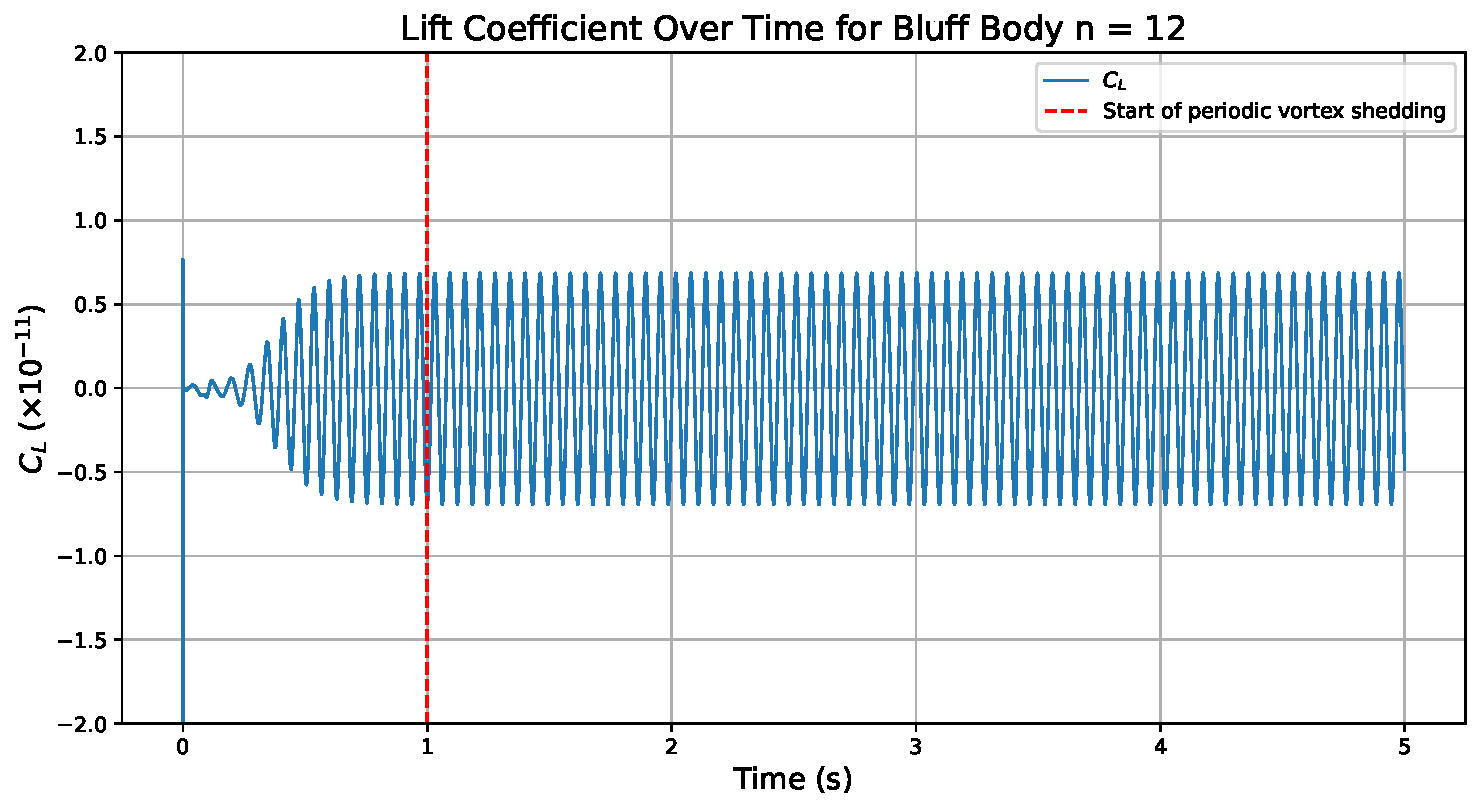
\includegraphics[width=\textwidth]{images/12face_graph}
	\caption{Lift coefficient $C_L$ over time for the bluff body $n=12$. The red dashed line indicates the start of the steady-state phase at $t = 1\,\mathrm{s}$.}
	\label{fig:12FaceGraph} 
\end{figure}

\subsubsection{Sample Calculation of Vortex Shedding Frequency for Bluff Body $n=2$ using Python}

\begin{figure}[H]
	\centering
	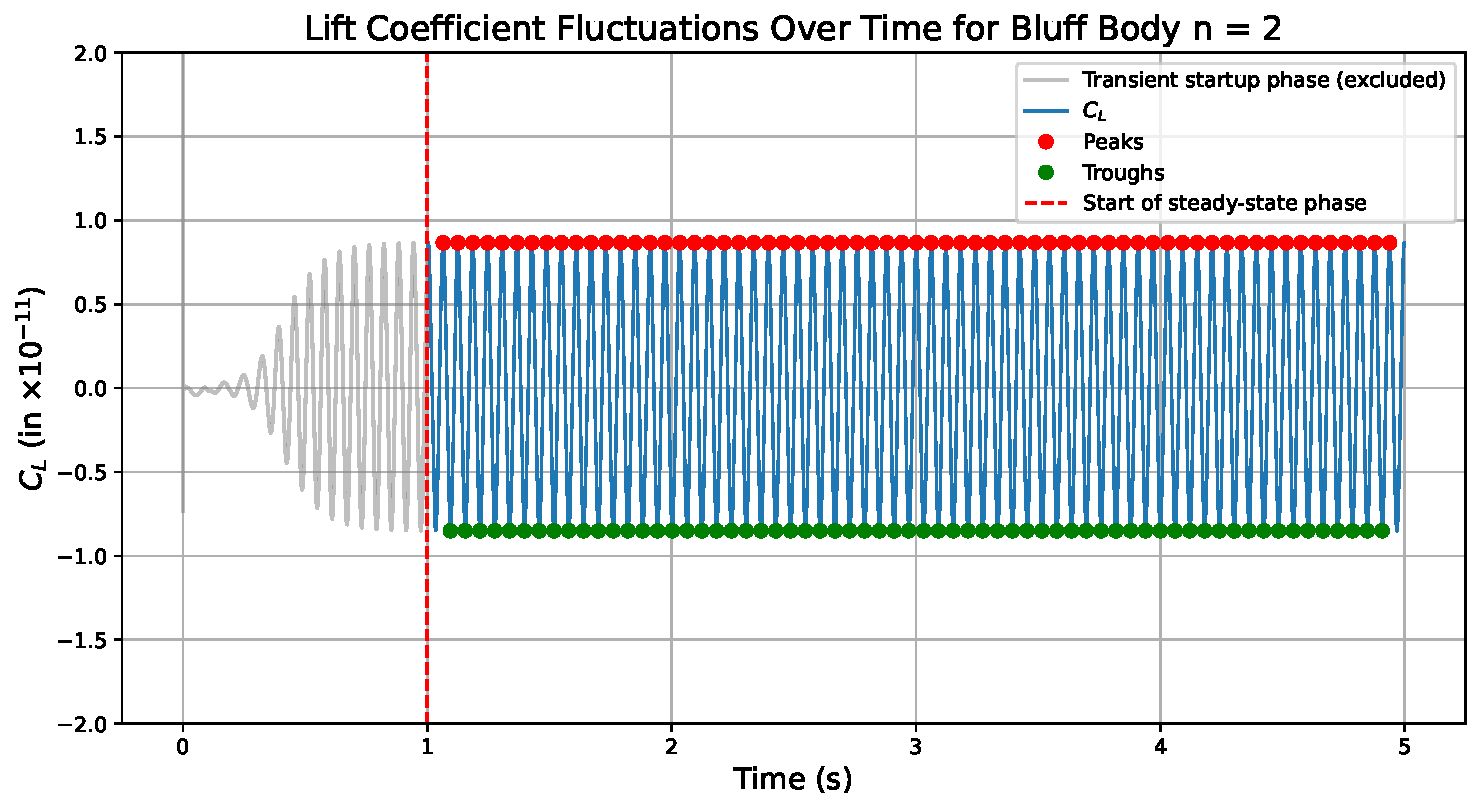
\includegraphics[width=\textwidth]{images/2face_graph_sample_Calc}
	\caption{Sample visualization of the peaks and troughs identification on the Lift Coefficient $C_L$ over time graph for bluff body $n=2$. The transient startup, colored in gray, is excluded from the detection.}
	\label{fig:2FaceGraphSampleCalc} 
\end{figure}

\begin{tcolorbox}[title=Python Output,fonttitle=\bfseries,
	colframe=black!75!white,colback=gray!10!white,boxrule=0.5pt,
	fontupper=\ttfamily]
	Number of peaks:    65 \\
	Number of troughs:  64 \\
	
	Average time period: 0.06052 s \\
\end{tcolorbox}

Using the outputted average period \( T = 0.06052 \, \text{s} \), the vortex shedding frequency was calculated with:

\[
f = \frac{1}{T} = \frac{1}{0.06052} = 16.52346 \, Hz
\]

This represents the vortex shedding frequency of the bluff body with \( n = 2 \) faces in steady-state laminar flow.

\subsubsection{A Comparison of Vortex Shedding Frequency with Varying $n$}

\begin{figure}[H]
	\centering
	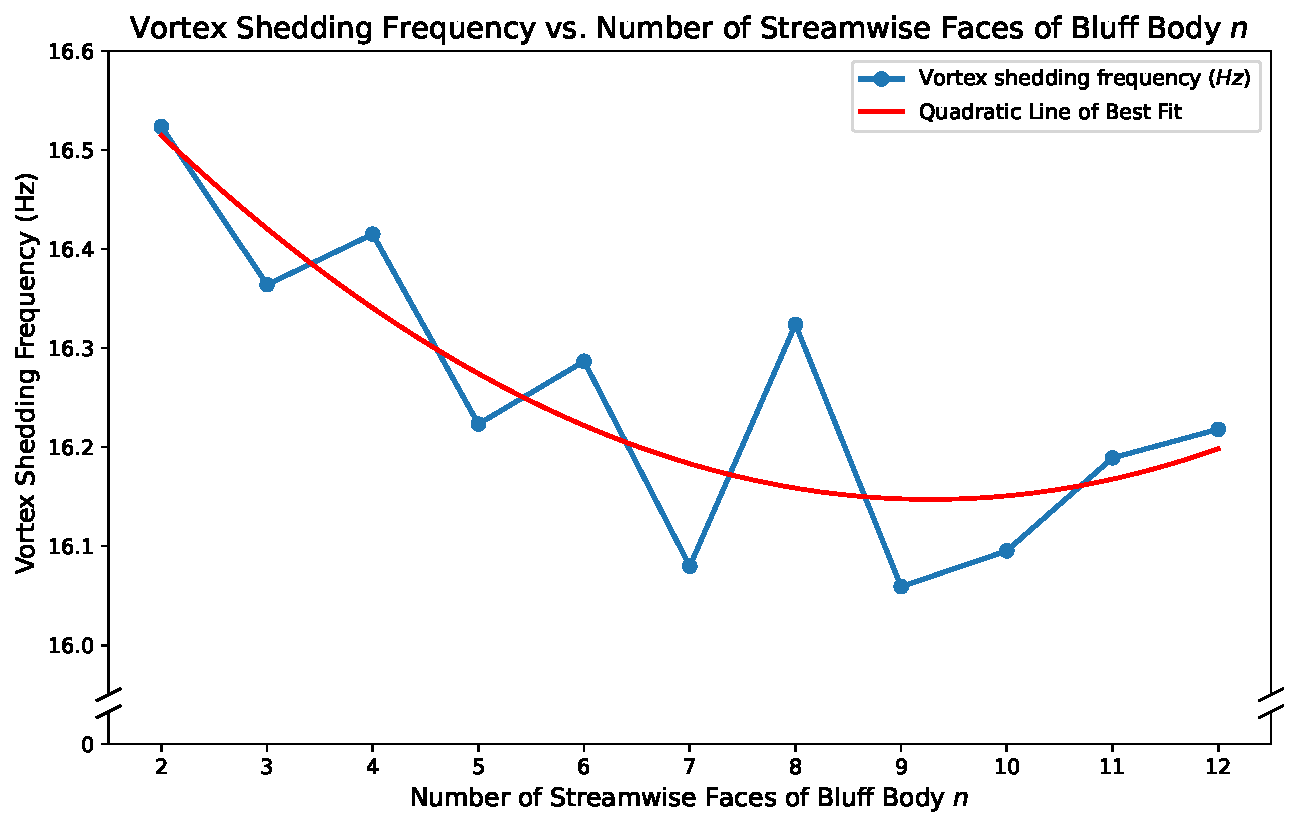
\includegraphics[width=\textwidth]{images/overall}
	\caption{}
	\label{fig:overall} 
\end{figure}


\subsection{Results of Practical Investigation}
After review of the footage it was found that the flow regime exhibited in the flow tank was not laminar. Despite many attempts to achieve laminar flow, the flow remained turbulent, as demonstrated by the irregular wake patterns. Nevertheless, the experiment yielded qualitative value. The use of potassium permanganate crystals allowed for a clear visualization of the boundary layer, flow separation and vortex shedding formation of the different bluff bodies.


	
\foreach \n in {2,...,12} {
	\subsubsection*{Snapshots of the Practical Run of Bluff Body $n = \n$}
	\begin{figure}[H]
		\centering
		
		% === Row 1 ===
		\begin{subfigure}[t]{0.48\textwidth}
			\centering
			\includegraphics[width=\linewidth]{images/\n Face/\n Face_0s.jpg}
			\caption{Snapshot of bluff body $n = \n$ at time 0 seconds}
		\end{subfigure}
		\hfill
		\begin{subfigure}[t]{0.48\textwidth}
			\centering
			\includegraphics[width=\linewidth]{images/\n Face/\n Face_1s.jpg}
			\caption{Snapshot of bluff body $n = \n$ at time 1 second}
		\end{subfigure}
		
		\vspace{1em}
		
		% === Row 2 ===
		\begin{subfigure}[t]{0.48\textwidth}
			\centering
			\includegraphics[width=\linewidth]{images/\n Face/\n Face_2s.jpg}
			\caption{Snapshot of bluff body $n = \n$ at time 2 seconds}
		\end{subfigure}
		\hfill
		\begin{subfigure}[t]{0.48\textwidth}
			\centering
			\includegraphics[width=\linewidth]{images/\n Face/\n Face_3s.jpg}
			\caption{Snapshot of bluff body $n = \n$ at time 3 seconds}
		\end{subfigure}
		
		\vspace{1em}
		
		% === Row 3 ===
		\begin{subfigure}[t]{0.48\textwidth}
			\centering
			\includegraphics[width=\linewidth]{images/\n Face/\n Face_4s.jpg}
			\caption{Snapshot of bluff body $n = \n$ at time 4 seconds}
		\end{subfigure}
		\hfill
		\begin{subfigure}[t]{0.48\textwidth}
			\centering
			\includegraphics[width=\linewidth]{images/\n Face/\n Face_5s.jpg}
			\caption{Snapshot of bluff body $n = \n$ at time 5 seconds}
		\end{subfigure}
		
	\end{figure}
}


	
	
	
	





\section{Conclusion}
The goal of this study was to investigate how the number of streamwise faces $n$ of a bluff body influence the vortex shedding frequency in laminar flow. Bluff bodies ranging from $n = 1 \text{\textendash\ } 12$ were analyzed both theoretically and practically. However, as stated in \Cref{sec:resultsPractical}, only the theoretical investigation yielded results of significance to fulfill the aim. 

The research question was thoroughly explored by theoretical means using OpenFOAM simulations, allowing for precise measurements of the fluctuations of the lift coefficient, and, in turn, an accurate determination of the vortex shedding frequency, using a time step based approach. Although the practical component of this investigation failed to achieve laminar flow conditions, it provided beneficial visual insight into the mechanism of vortex shedding, enhancing the investigation's tangibility while aiding conceptual understanding.

It was found that there is an overall decrease in vortex shedding frequency as the number of streamwise faces $n$ of a bluff body increases \textemdash\ confirming the previously mentioned hypothesis. This trend is exemplified by bluff body $n = 2$ which produced a vortex shedding frequency of $16.52346\, Hz$, while the bluff body $n = 12$ produced a vortex shedding frequency of $16.21797\, Hz$. The overall trend is in agreement with literature such as \textcite{goncalves1999strouhal} which concluded that a higher number of streamwise faces leads to a decreased Strouhal number and therefore a decreased vortex shedding frequency.

A quadratic line of best fit produced an $R^2$ value of 0.70, indicating a moderate non-linear correlation between the number of streamwise faces $n$ and the vortex shedding frequency. The rather low $R^2$ value may be attributed to numerical uncertainties of the simulation due to various factors such as the mesh resolution \parencite{city7565}. However, quantifying these uncertainties is difficult due to potential mutually canceling effects. 





\printbibliography

\clearpage

\appendix
\addcontentsline{toc}{section}{Appendices}



\lstinputlisting[
caption={Calculating time period by identifying peaks and troughs of lift coefficient $C_L$ graph. The exact file paths were excluded due to privacy reasons},
label={lst:freqDetermination}
]{code/dataAnalysis.py}

	
\end{document}
